%!TEX program = xelatex
\documentclass[10pt, compress]{beamer}
\usepackage{array}
\usepackage{listings} % for code snippets
\usepackage{enumitem}
\usepackage{xltxtra}
\usepackage{xgreek}
\usepackage{multicol}
\usepackage{commath}
\usepackage{amsmath}
\usepackage[export]{adjustbox}
\usepackage{wrapfig}

\usepackage{subfig}
\renewcommand{\thesubfigure}{\roman{subfigure}}

% matlab
\usepackage{listings}
\usepackage{color} %red, green, blue, yellow, cyan, magenta, black, white
\definecolor{mygreen}{RGB}{28,172,0} % color values Red, Green, Blue
\definecolor{mylilas}{RGB}{170,55,241}
\setbeamercolor{background canvas}{bg=white}

% -------

\usefonttheme{serif} % this made greek work
\setmainfont[Mapping=tex-text]{Liberation Serif}
\usetheme{metropolis}


\begin{document}

\begin{frame}
\thispagestyle{empty}

\begin{flushleft}
% \begin{figure}
%   
\includegraphics[width=.6\linewidth, left]{imgs/square-official-800}
% \end{figure}
\end{flushleft}
\Large{\textbf{Deep Learning Workshop}} \\
% \vspace*{-.05cm}

% \fontsize{10pt}{Εργαστήριο 1 \\ Εισαγωγή στα Σήματα \& Συστήματα με Matlab}
% {\fontsize{12}{40} \selectfont ``A.I. is the new electricity"} \\
% {\fontsize{9}{40} \selectfont \qquad \qquad \qquad \qquad \qquad -Andrew NG} \\
\begin{multicols}{2}
{\fontsize{10}{40} \selectfont ``...what we want is a machine} \\
\vspace*{-.3cm}
{\fontsize{10}{40} \selectfont that can learn from experience."} \\
\vspace*{-.3cm}
{\fontsize{8}{40} \selectfont  \qquad \qquad \qquad \qquad Alan Turing, 1947} \\
% \hrulefill \\

\columnbreak
\vspace*{-1.4cm}

\begin{figure}
  
\includegraphics[width=.4\linewidth, right]{imgs/square-official-800}
\end{figure}
\end{multicols}
\vspace{-1.1cm}
\hrulefill \\
{\fontsize{10}{40} \selectfont Xenofon Karagiannis} \\

% \vspace*{.5cm}
% \begin{figure}
%   \includegraphics[width=.6\linewidth]{imgs/logo-fixed-1}
% \end{figure}
\end{frame}

\setcounter{framenumber}{0}

\begin{frame}
  \vspace{.6cm}
  \textbf{This workshop...} \\
  theory \\
  hands on \\
  applications \\
  thesis \\
\end{frame}

\begin{frame}
  \vspace{.6cm}
  \textbf{Goals} \\
  solid under
\end{frame}

\begin{frame}
  % \vspace{.6cm}
  \begin{center}
  \makebox[\textwidth]{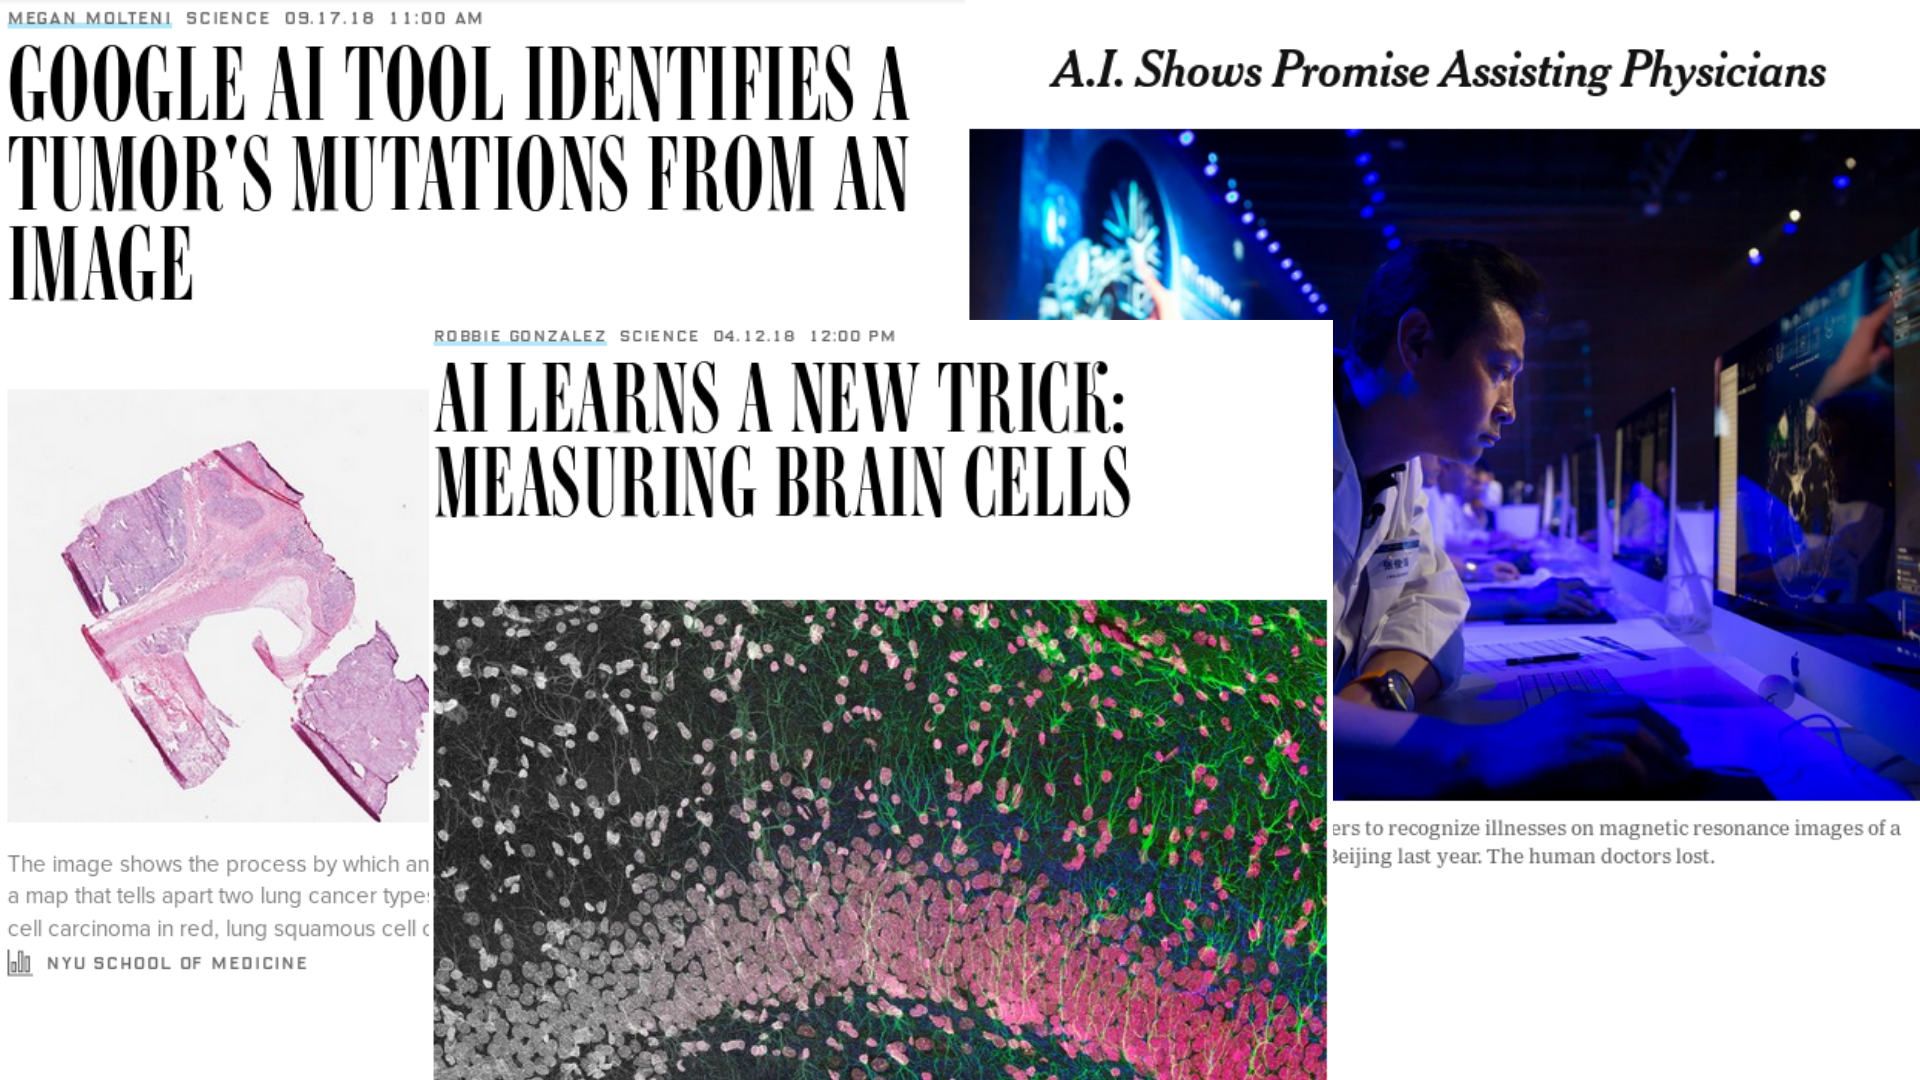
\includegraphics[width=.95\paperwidth]{imgs/news/1}}
  \end{center}
\end{frame}

\begin{frame}
  % \vspace{.6cm}
  \begin{center}
  \makebox[\textwidth]{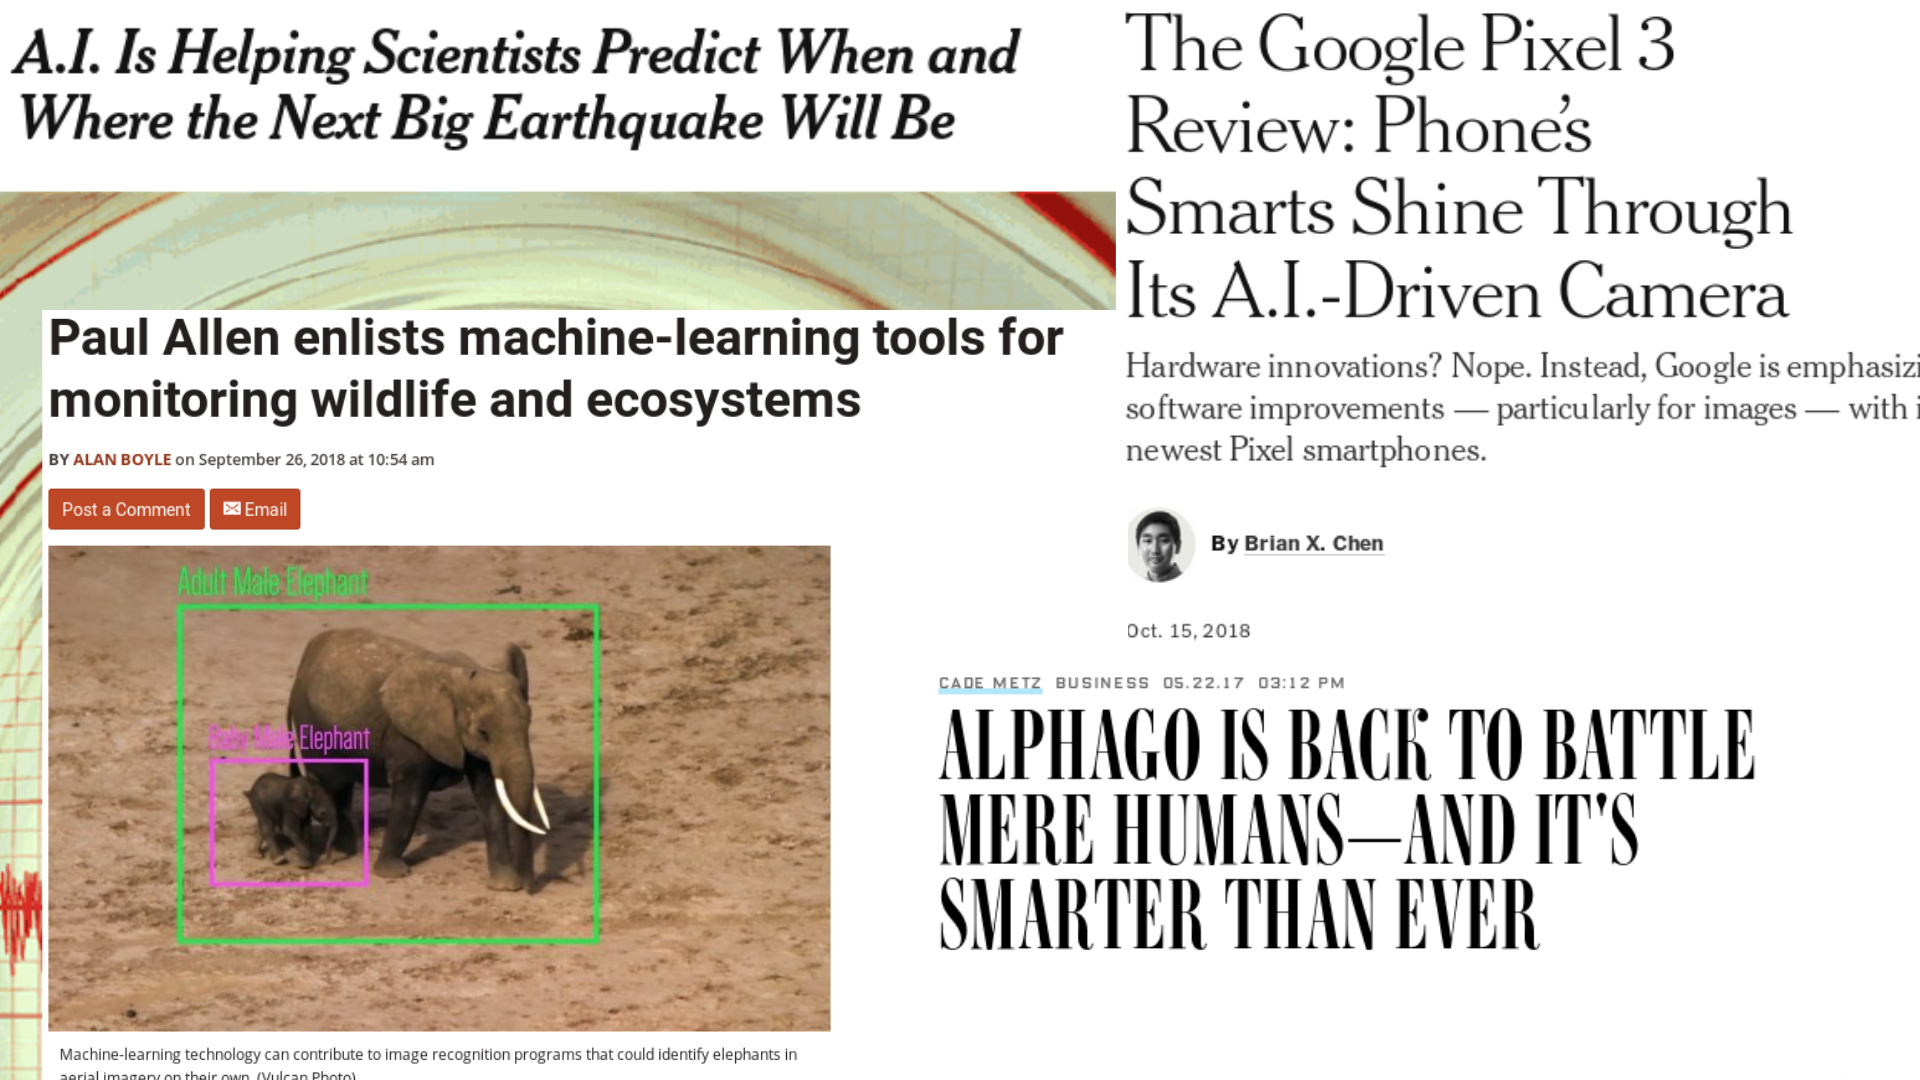
\includegraphics[width=.95\paperwidth]{imgs/news/2}}
  \end{center}
\end{frame}

% AI is the new electricity
\begin{frame}
  \vspace{.6cm}
  \textbf{``AI is the new electricity"} \\
  \qquad \qquad \qquad \small{\textit{Andrew NG}} \\

  \vspace{.6cm}
  \begin{figure}
    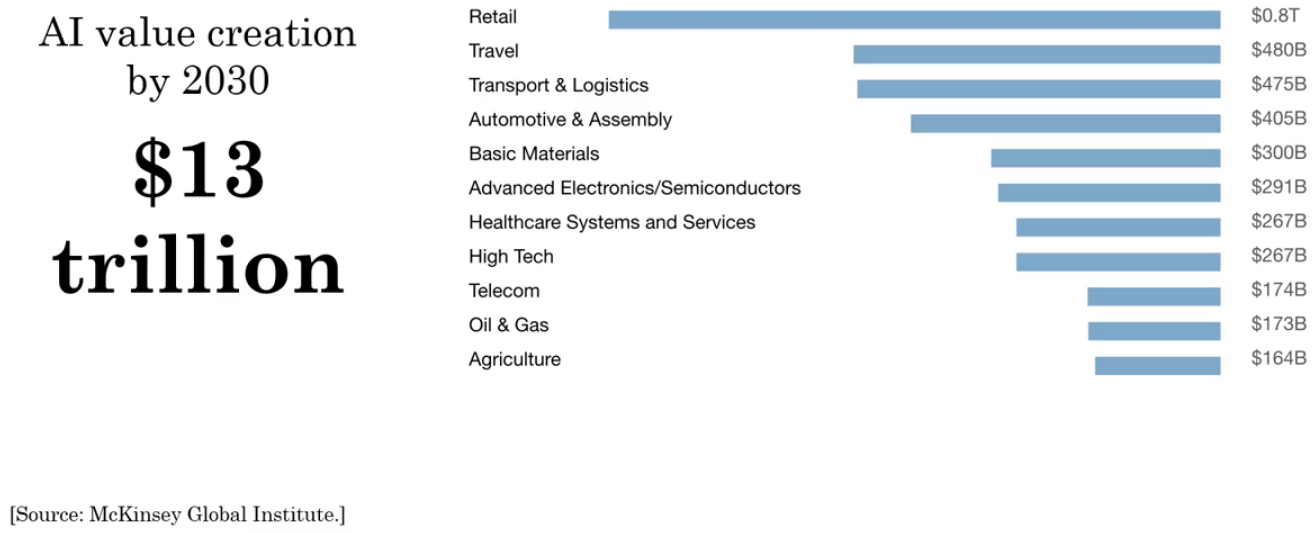
\includegraphics[width=1\linewidth]{imgs/ai_for_everyone_course/1}
  \end{figure}
\end{frame}

% Buzzwords
\begin{frame}
  \vspace{.4cm}

  \begin{figure}
    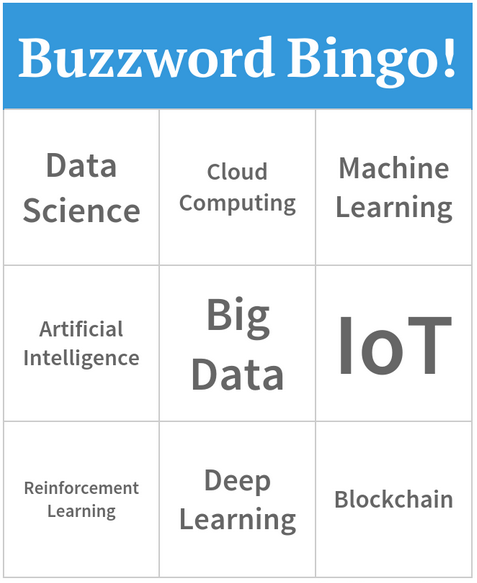
\includegraphics[width=.64\linewidth]{imgs/buzzwords}
  \end{figure}
\end{frame}

% Definitions
\begin{frame}
  \begin{multicols}{2}
  \textbf{Machine Learning}

  ``Field of study that gives computers the ability to learn without being explicitly programmed."

  -Arthur Samuel (1959)

  \columnbreak

  \textbf{Data Science}

  Science of extracting knowledge and insights from data.


  \end{multicols}

  \begin{multicols}{2}
    \textit{An ML projects results in a piece of software that runs.}

    \columnbreak

    \textit{A Data Science projects is often a presentation that summarizes conclusions for executives to take business actions or that summarizes conclusions for a product team to decide how to improve a website.}

  \end{multicols}
\end{frame}

% Definitions
\begin{frame}
  \begin{multicols}{2}
  \textbf{Artificial Intelligence} \\ \hfill \break

  ``the study and design of intelligent agents" where an intelligent agent is a system that perceives its environment and takes actions which maximizes its chances of success.

  \columnbreak

  \begin{figure}
    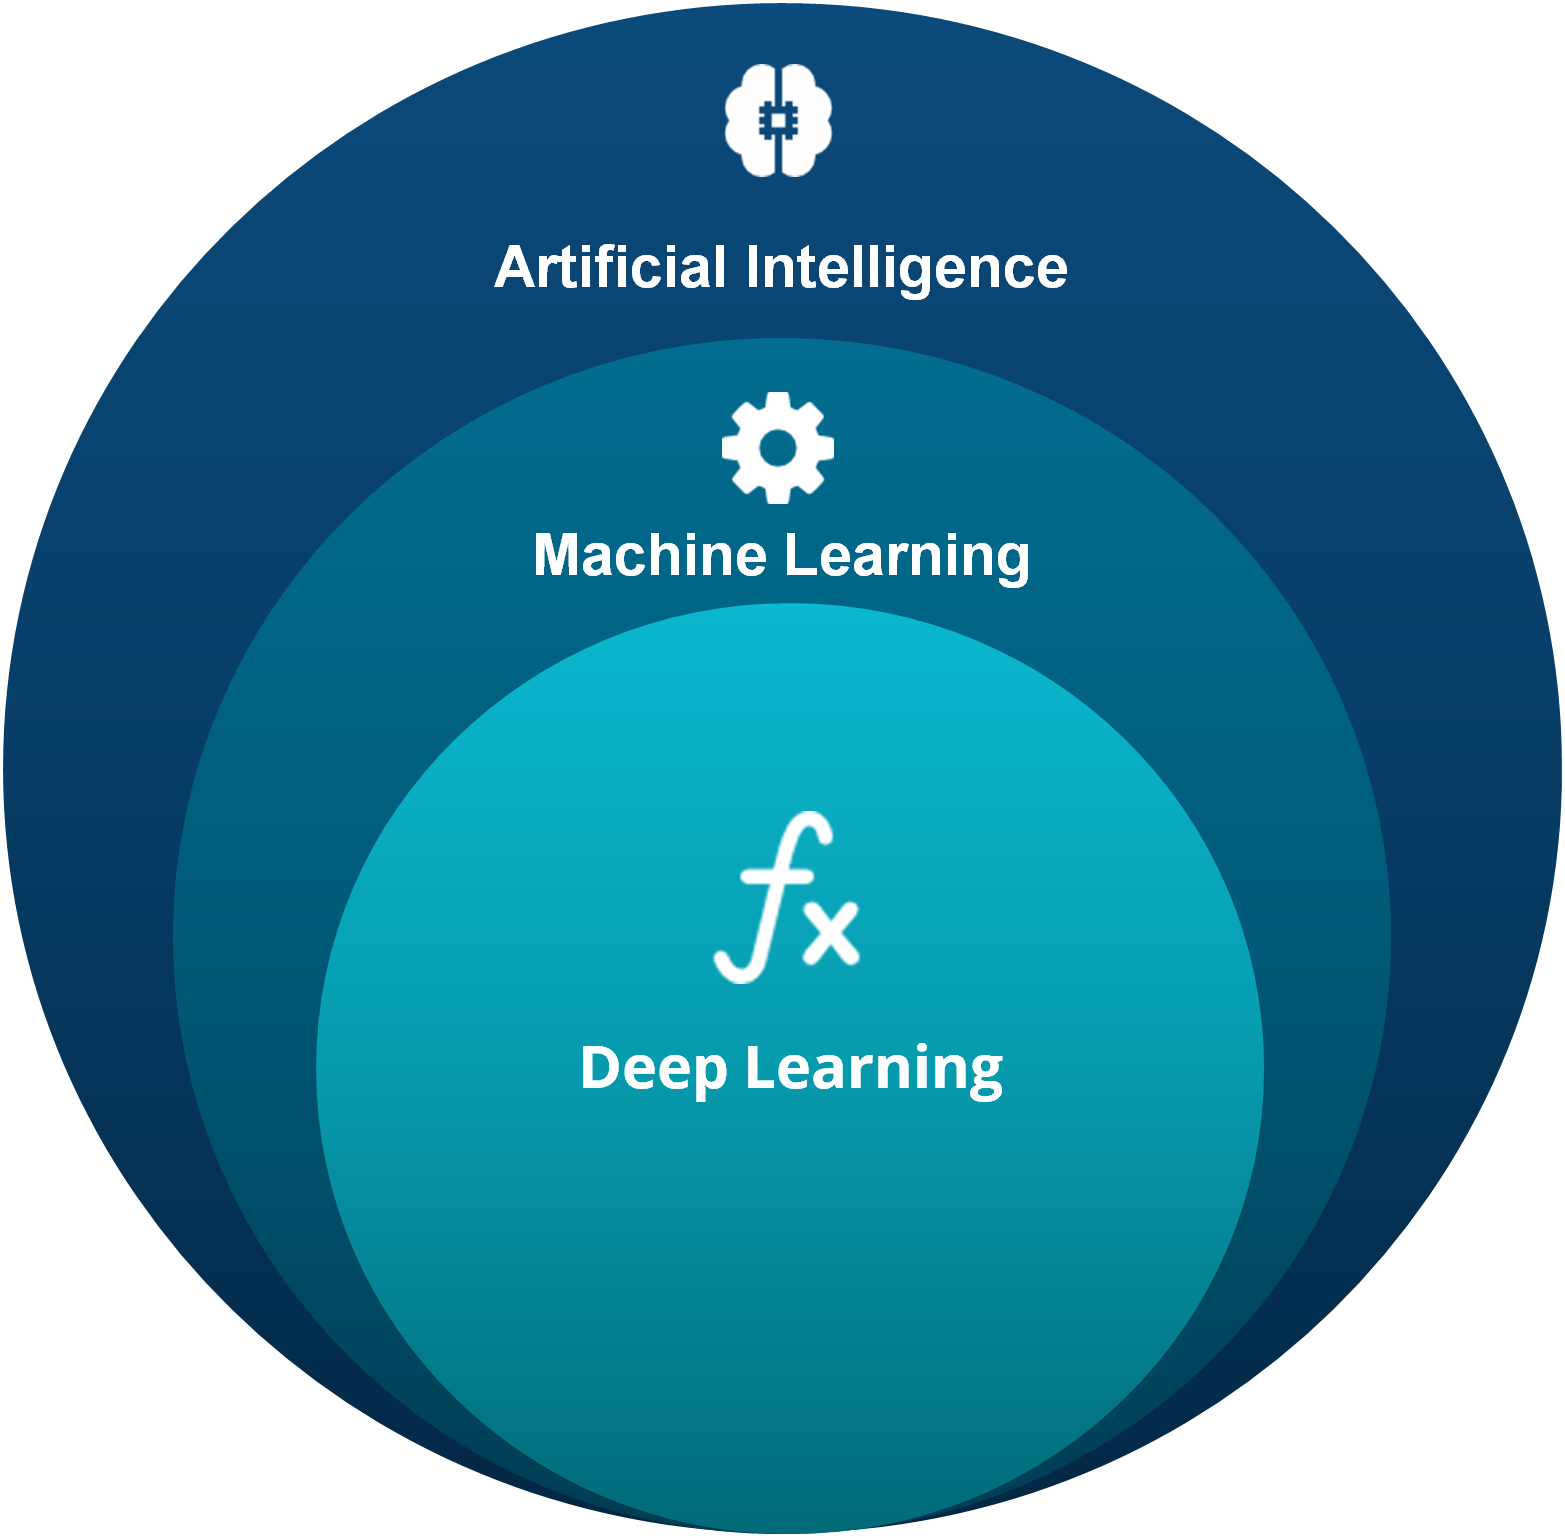
\includegraphics[width=.9\linewidth]{imgs/venn_ai_ml_dl}
  \end{figure}

  \end{multicols}
\end{frame}

\begin{frame}
  \begin{figure}
    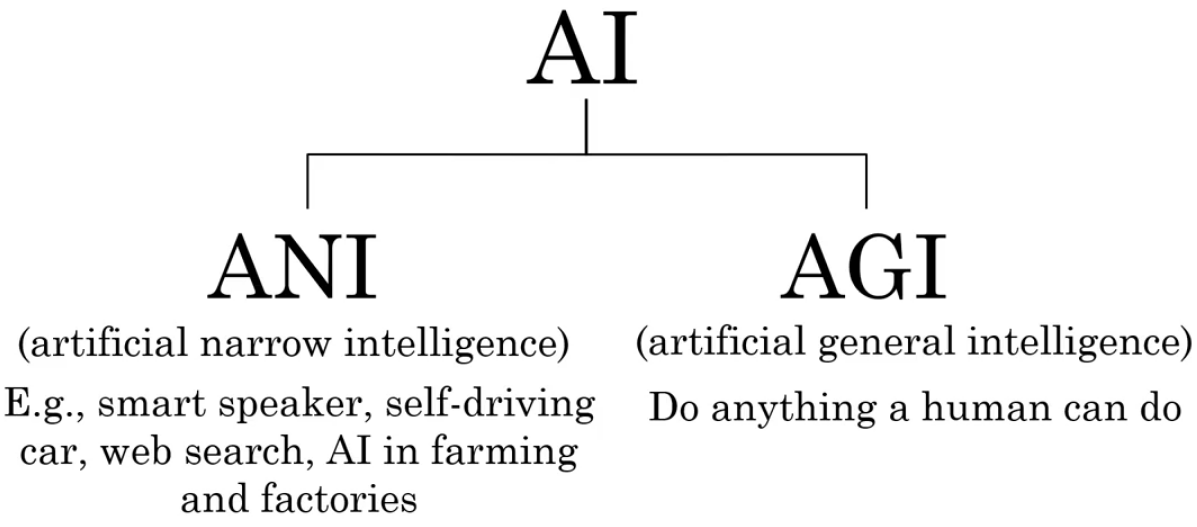
\includegraphics[width=.9\linewidth]{imgs/ai_for_everyone_course/2}
  \end{figure}
\end{frame}

% Color Restoration
\begin{frame}
  \vspace{.6cm}
  \textbf{Color Restoration} [\href{http://iizuka.cs.tsukuba.ac.jp/projects/colorization/data/colorization_sig2016.pdf}{link}] \\
  \small{Automatic colorization and color restoration in black and white images.} \\
  \vspace{.6cm}
  \begin{figure}
    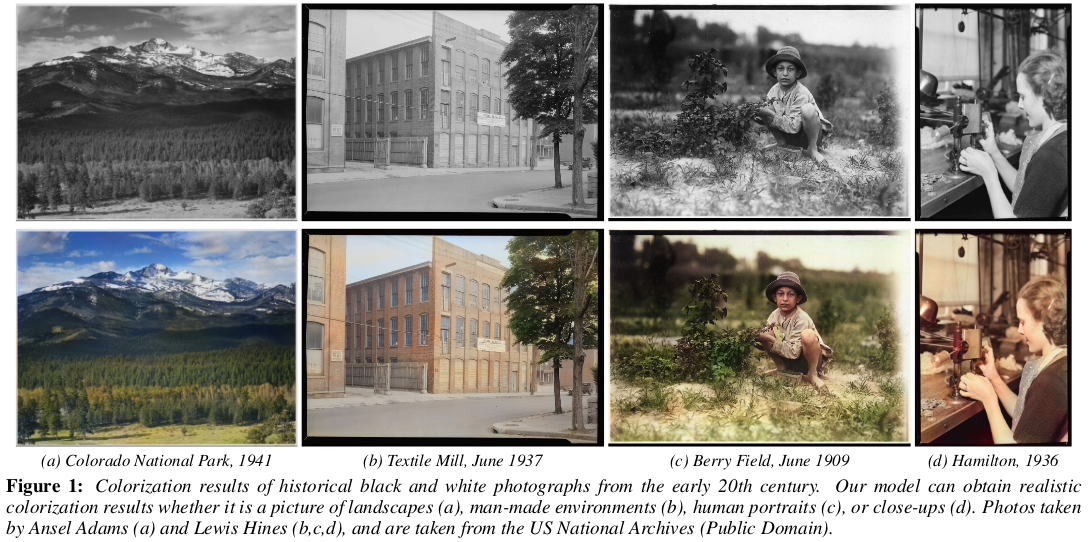
\includegraphics[width=1\linewidth]{imgs/edx_dl_keras/1}
  \end{figure}
\end{frame}

% Speech Reenactment
\begin{frame}
  \vspace{.6cm}
  \textbf{Speech Reenactment} [\href{https://grail.cs.washington.edu/projects/AudioToObama/}{link}] \\
  \small{Synthesizing Obama: Learning Lip Sync from Audio.} \\

  \vspace{.6cm}
  \begin{figure}
    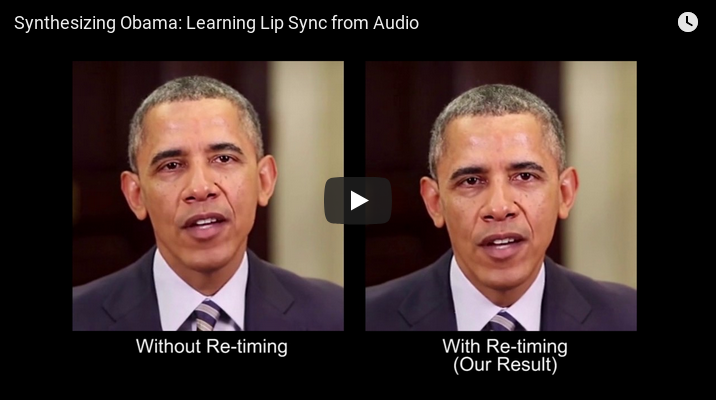
\includegraphics[width=1\linewidth]{imgs/edx_dl_keras/6}
  \end{figure}
\end{frame}

% Diagnose crop diseases
\begin{frame}
  \vspace{.6cm}
  \textbf{Diagnose crop diseases} [\href{https://www.youtube.com/watch?v=NlpS-DhayQA}{link}] \\

  \vspace{.6cm}
  \begin{figure}
    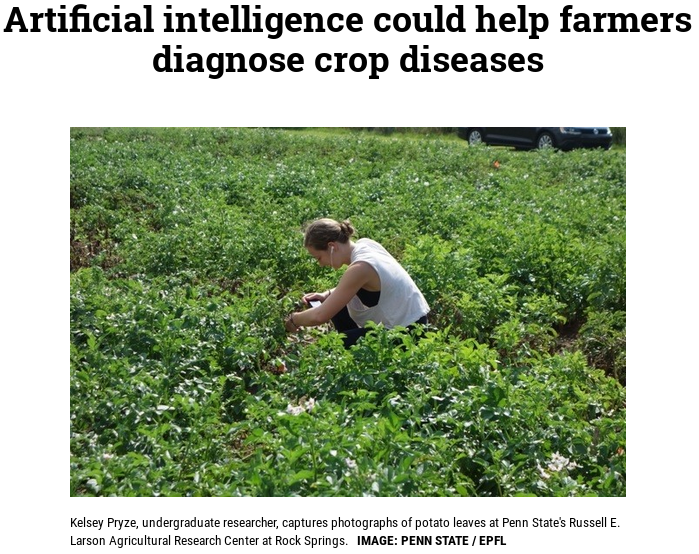
\includegraphics[width=.7\linewidth]{imgs/edx_dl_keras/7}
  \end{figure}
\end{frame}

% Car Vehicle / Traffic Lights / Pedestrian detection with YOLO
\begin{frame}
  \vspace{.6cm}
  \textbf{Car Vehicle / Traffic Lights / Pedestrian detection with YOLO} [\href{https://www.youtube.com/watch?v=OksuVuNY5o0}{link}] \\

  \vspace{.6cm}
  \begin{figure}
    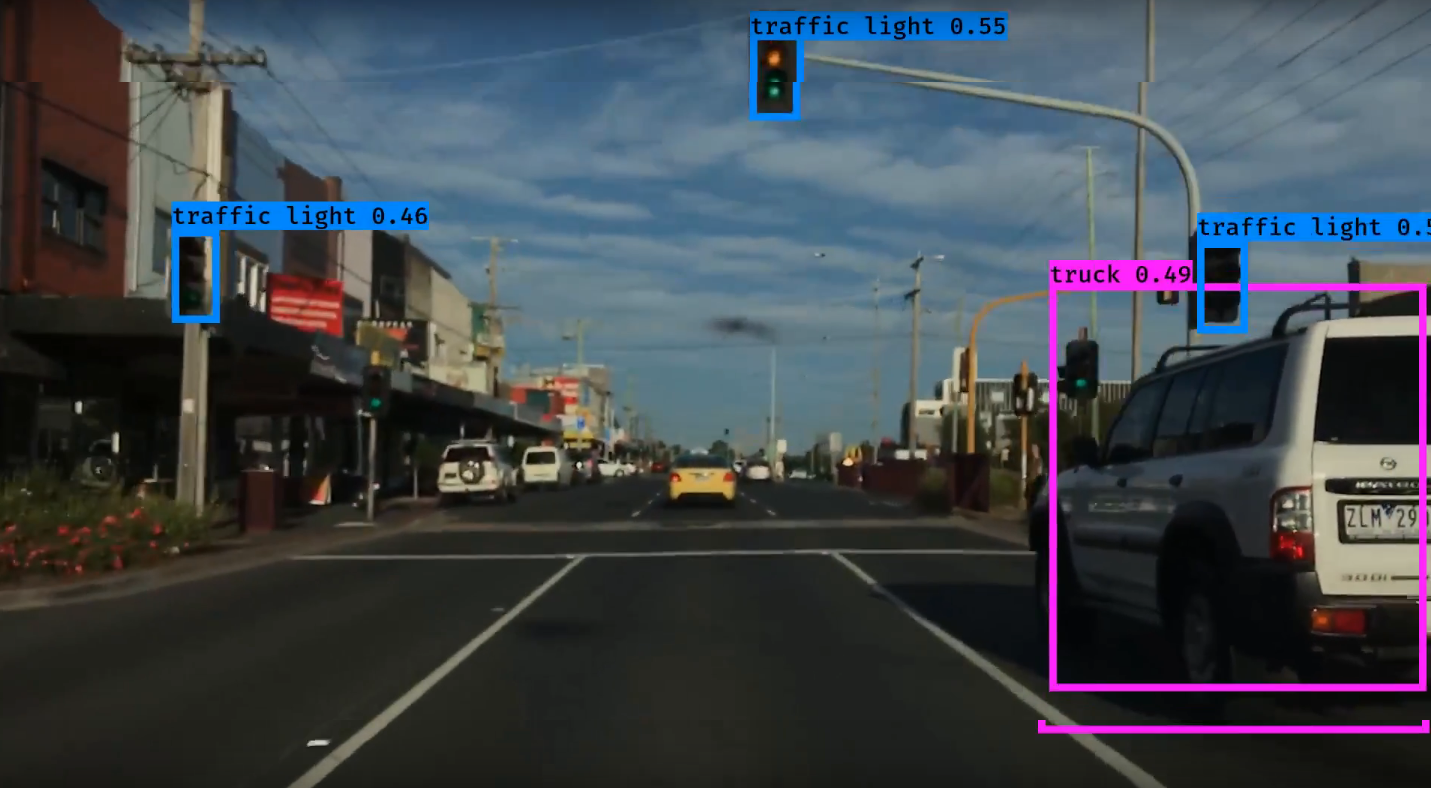
\includegraphics[width=.85\linewidth]{imgs/edx_dl_keras/8}
  \end{figure}
\end{frame}

% NVIDIA Invents AI Interactive Graphics
\begin{frame}
  \vspace{.6cm}
  \textbf{NVIDIA Invents AI Interactive Graphics} [\href{https://news.developer.nvidia.com/nvidia-invents-ai-interactive-graphics/}{link}] \\

  \vspace{.6cm}
  \begin{figure}
    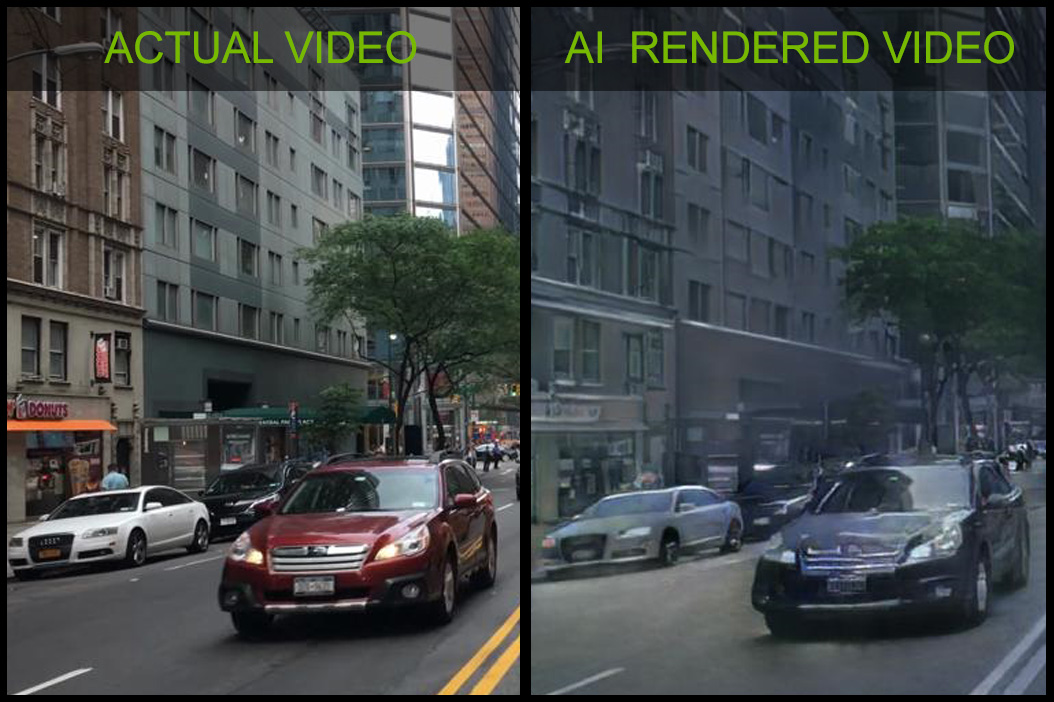
\includegraphics[width=.9\linewidth]{imgs/news/nvidia_1}
  \end{figure}
\end{frame}

\begin{frame}
  \vspace{.6cm}
  \textbf{Real Time Object Detection in 4K Video - RetinaNet} [\href{https://www.youtube.com/watch?v=KYueHEMGRos}{link}] \\

  \vspace{.6cm}
  \begin{figure}
    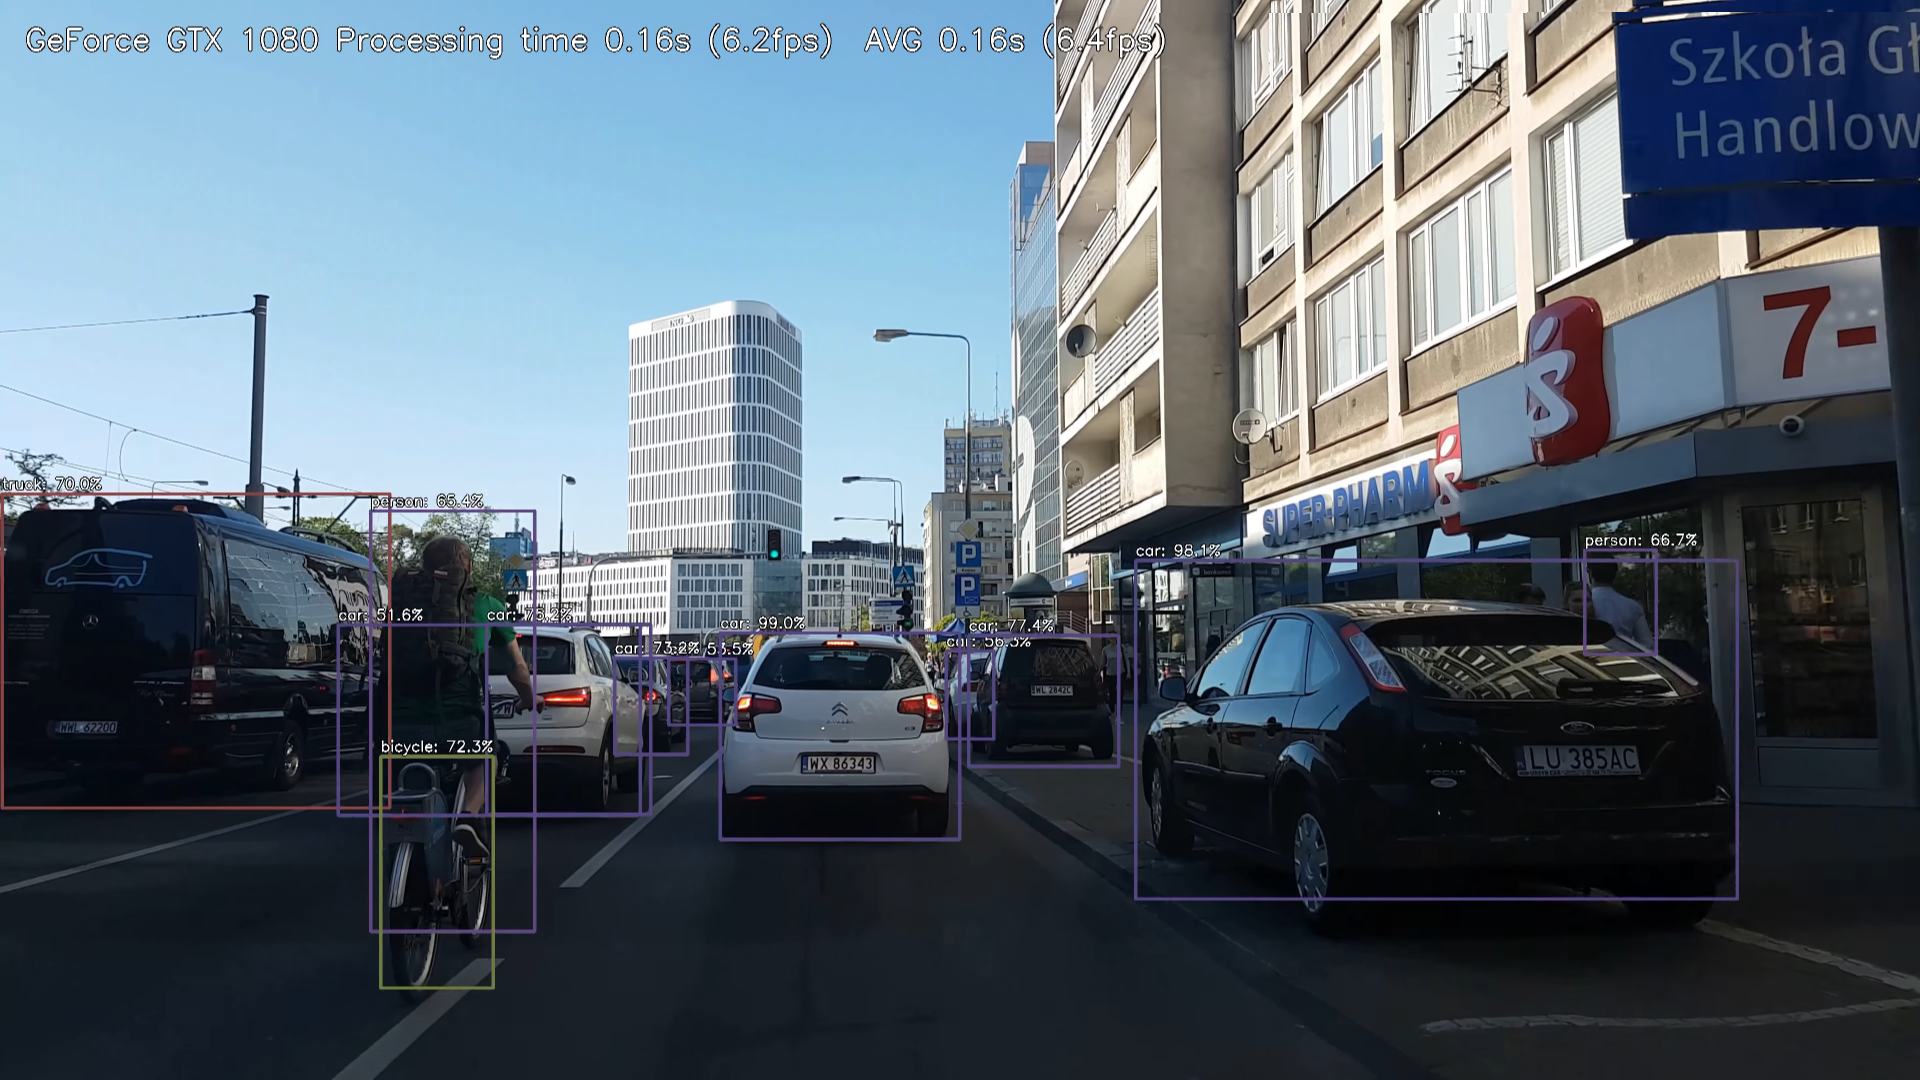
\includegraphics[width=.9\linewidth]{imgs/news/4k-retinanet}
  \end{figure}
\end{frame}

\begin{frame}
  \vspace{.6cm}
  \textbf{This person does not exist - GAN} [\href{https://thispersondoesnotexist.com/}{link}] \\

  \vspace{.6cm}
  \begin{figure}
    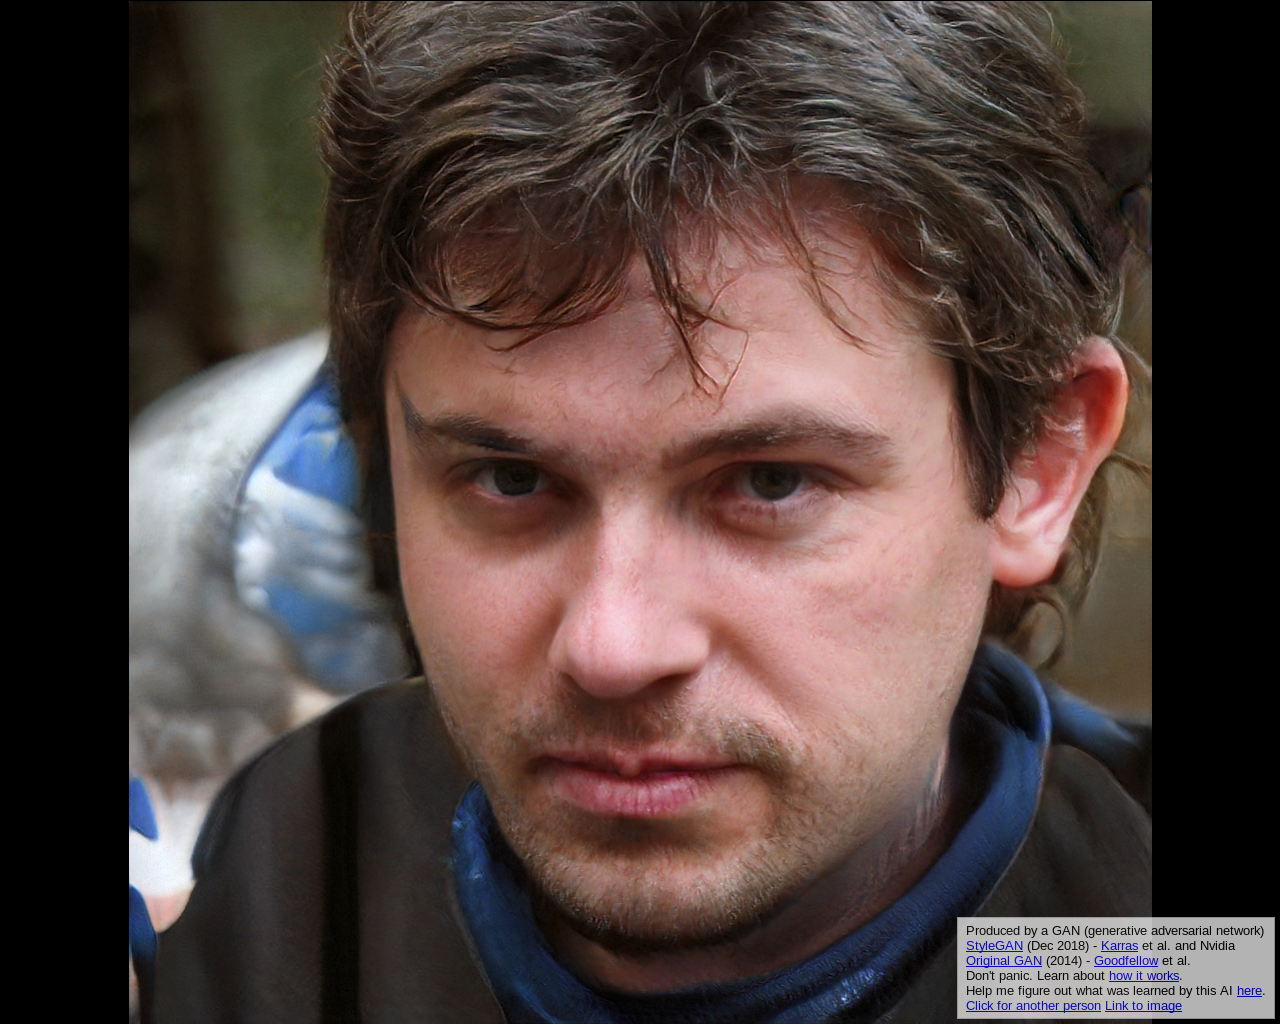
\includegraphics[width=.75\linewidth]{imgs/news/person}
  \end{figure}
\end{frame}

\begin{frame}
  \vspace{.6cm}
  \textbf{Google Doodle - Celebrating Johann Sebastian Bach} [\href{https://www.google.com/doodles/celebrating-johann-sebastian-bach}{link}] \\

  \vspace{.6cm}
  \begin{figure}
    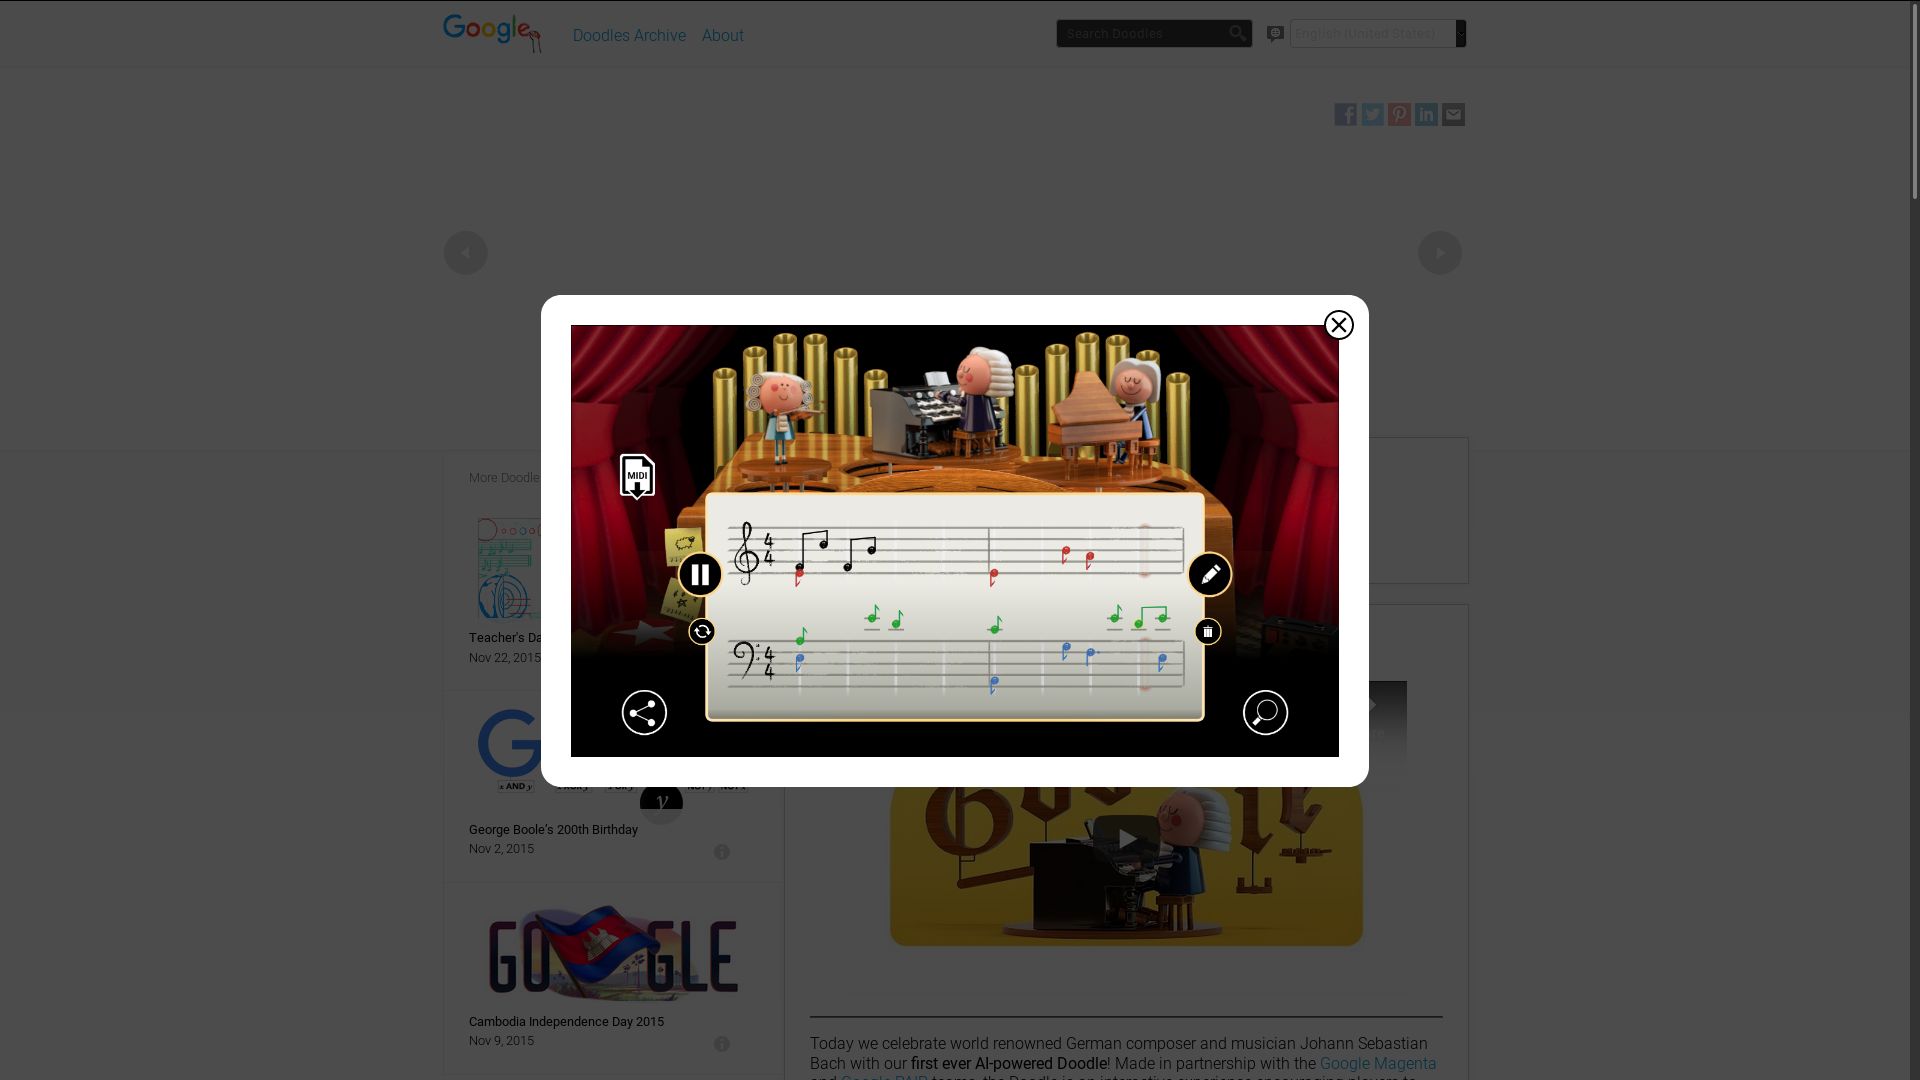
\includegraphics[width=.9\linewidth]{imgs/news/doodle}
  \end{figure}
\end{frame}

\begin{frame}
  \vspace{.6cm}
  \textbf{Google DeepMind - AlphaGo} [\href{https://deepmind.com/research/alphago/}{link}] \\

  \vspace{.6cm}
  \begin{figure}
    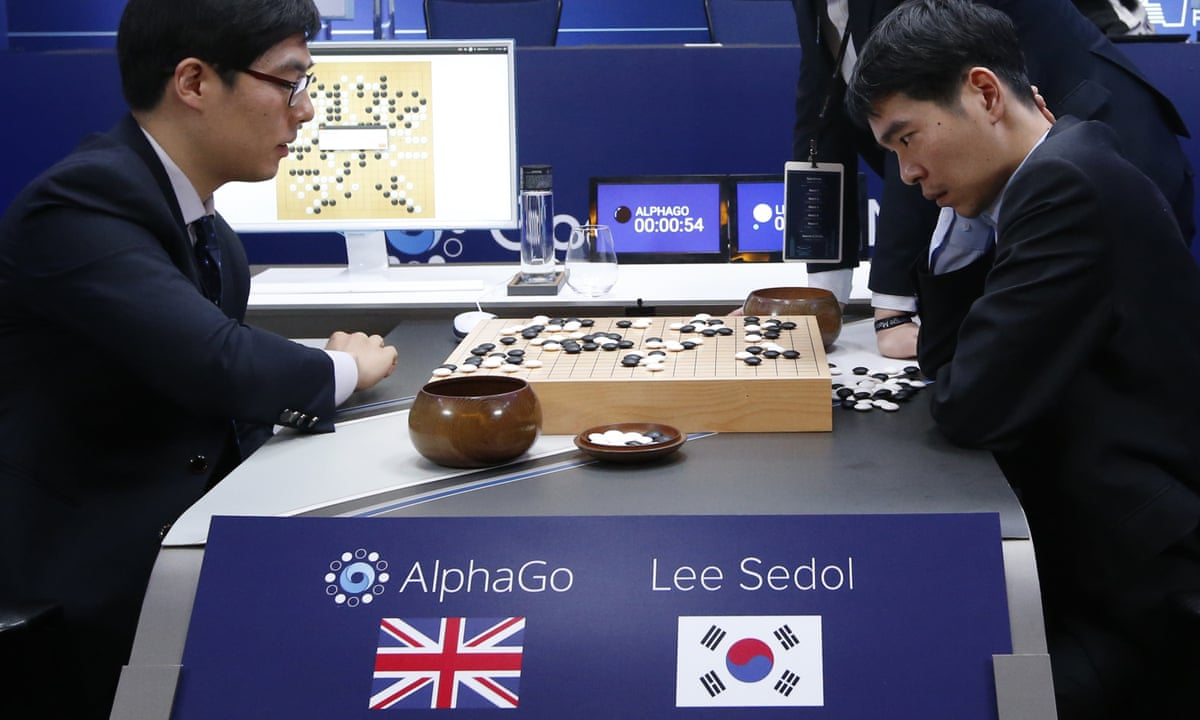
\includegraphics[width=.9\linewidth]{imgs/news/alphago}
  \end{figure}
\end{frame}

\begin{frame}
  \vspace{.6cm}
  \textbf{Google DeepMind - AlphaStar Starcraft II} [\href{https://deepmind.com/blog/alphastar-mastering-real-time-strategy-game-starcraft-ii/}{link}] \\

  \vspace{.6cm}
  \begin{figure}
    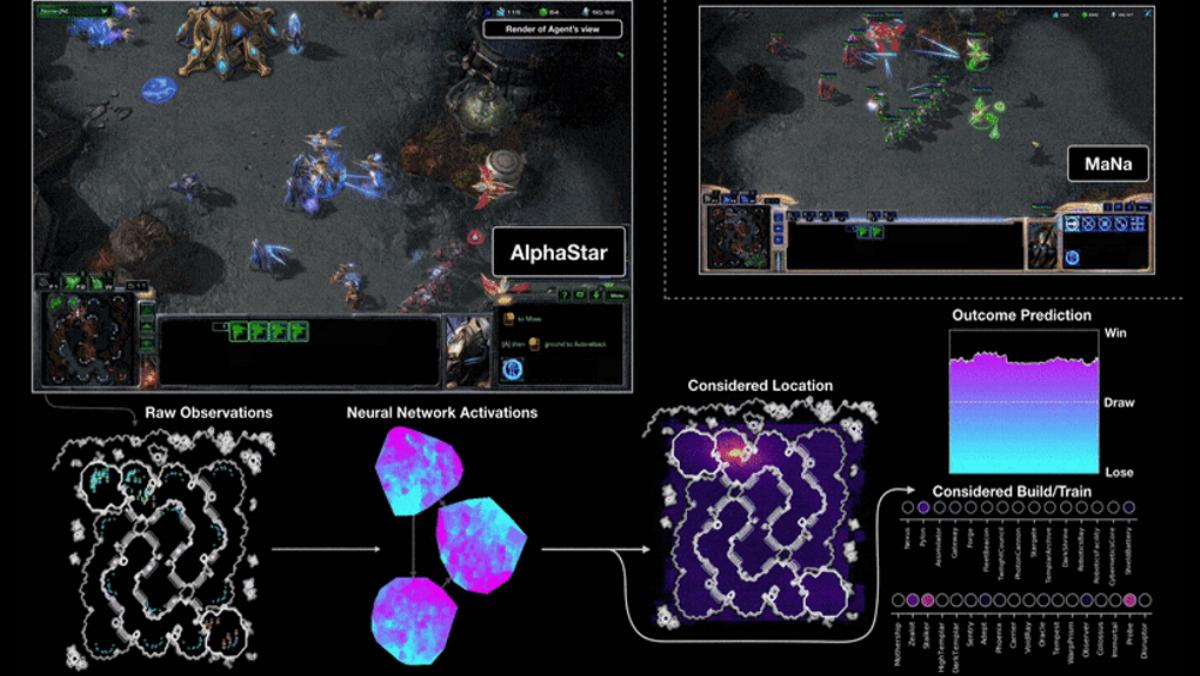
\includegraphics[width=.9\linewidth]{imgs/news/alphastar}
  \end{figure}
\end{frame}

\begin{frame}
  \vspace{.6cm}
  \textbf{OpenAI Dota2} [\href{https://openai.com/blog/dota-2/}{link}] \\

  \vspace{.6cm}
  \begin{figure}
    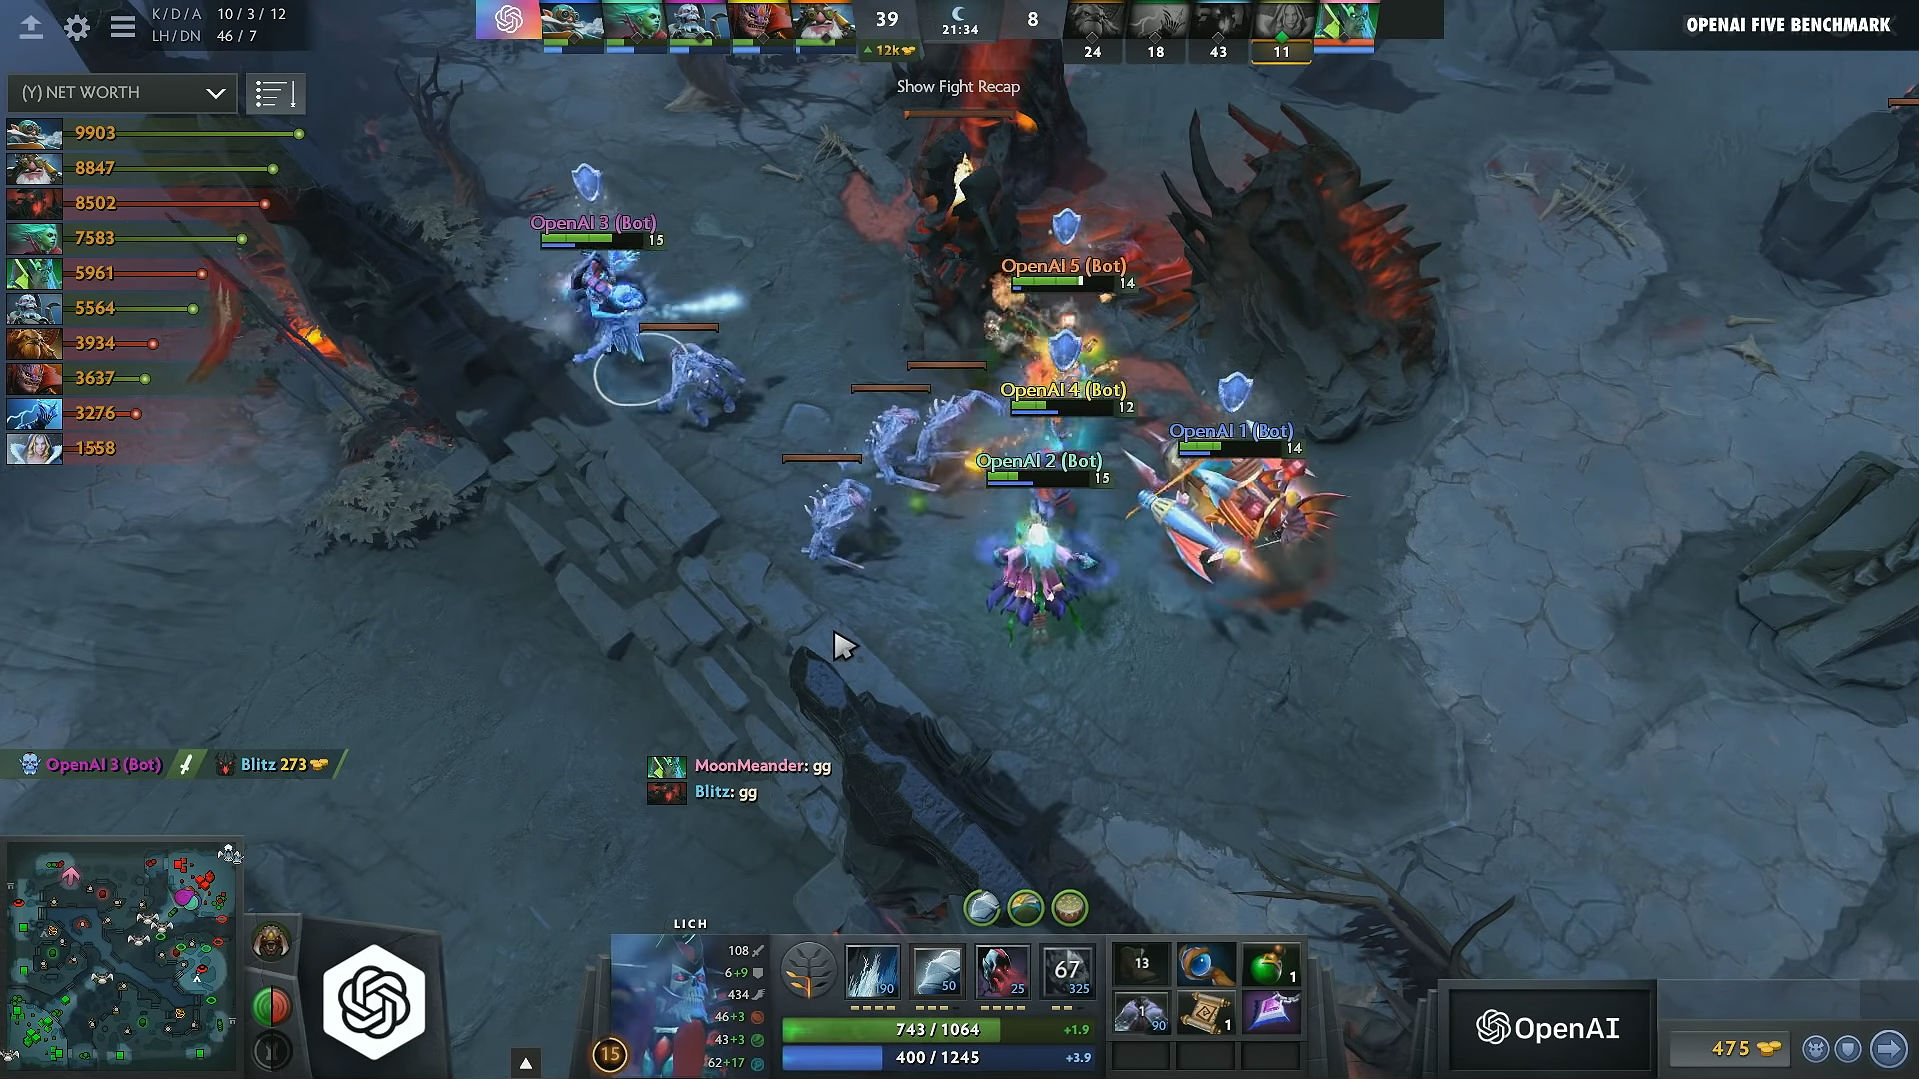
\includegraphics[width=.9\linewidth]{imgs/news/openai}
  \end{figure}
\end{frame}

% funny_1
\begin{frame}
  \vspace{.6cm}
  \begin{figure}
    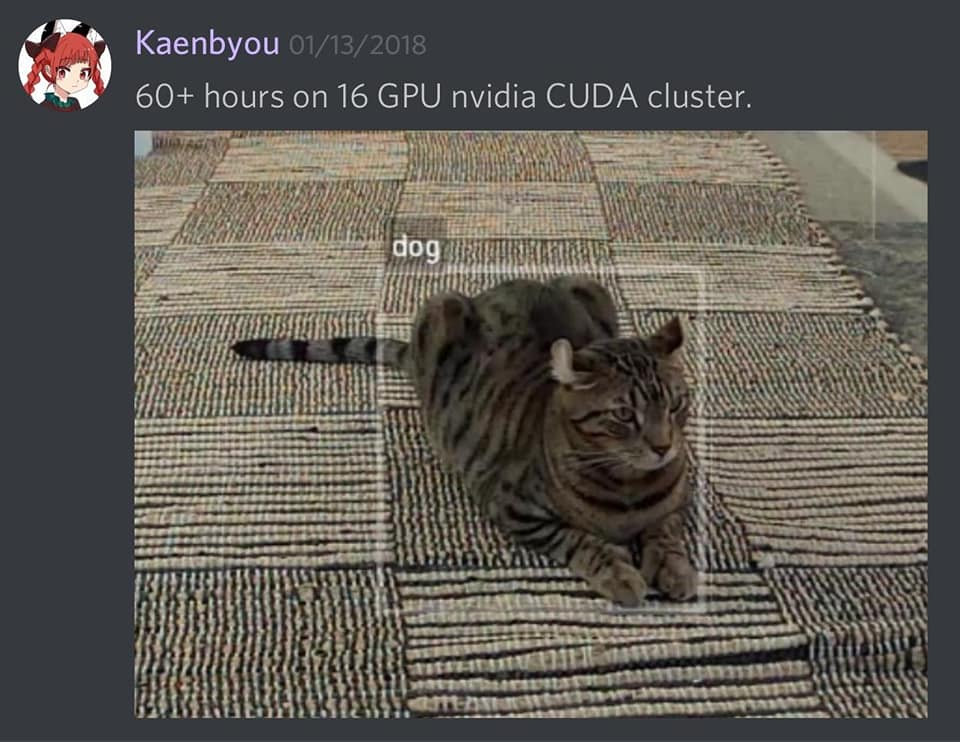
\includegraphics[width=.9\linewidth]{imgs/funny_1}
  \end{figure}
\end{frame}

% funny_2
\begin{frame}
  \vspace{.3cm}
  \begin{figure}
    
\includegraphics[width=.6\linewidth]{imgs/funny_2}
  \end{figure}
\end{frame}

% timeline
\begin{frame}
\begin{figure}
  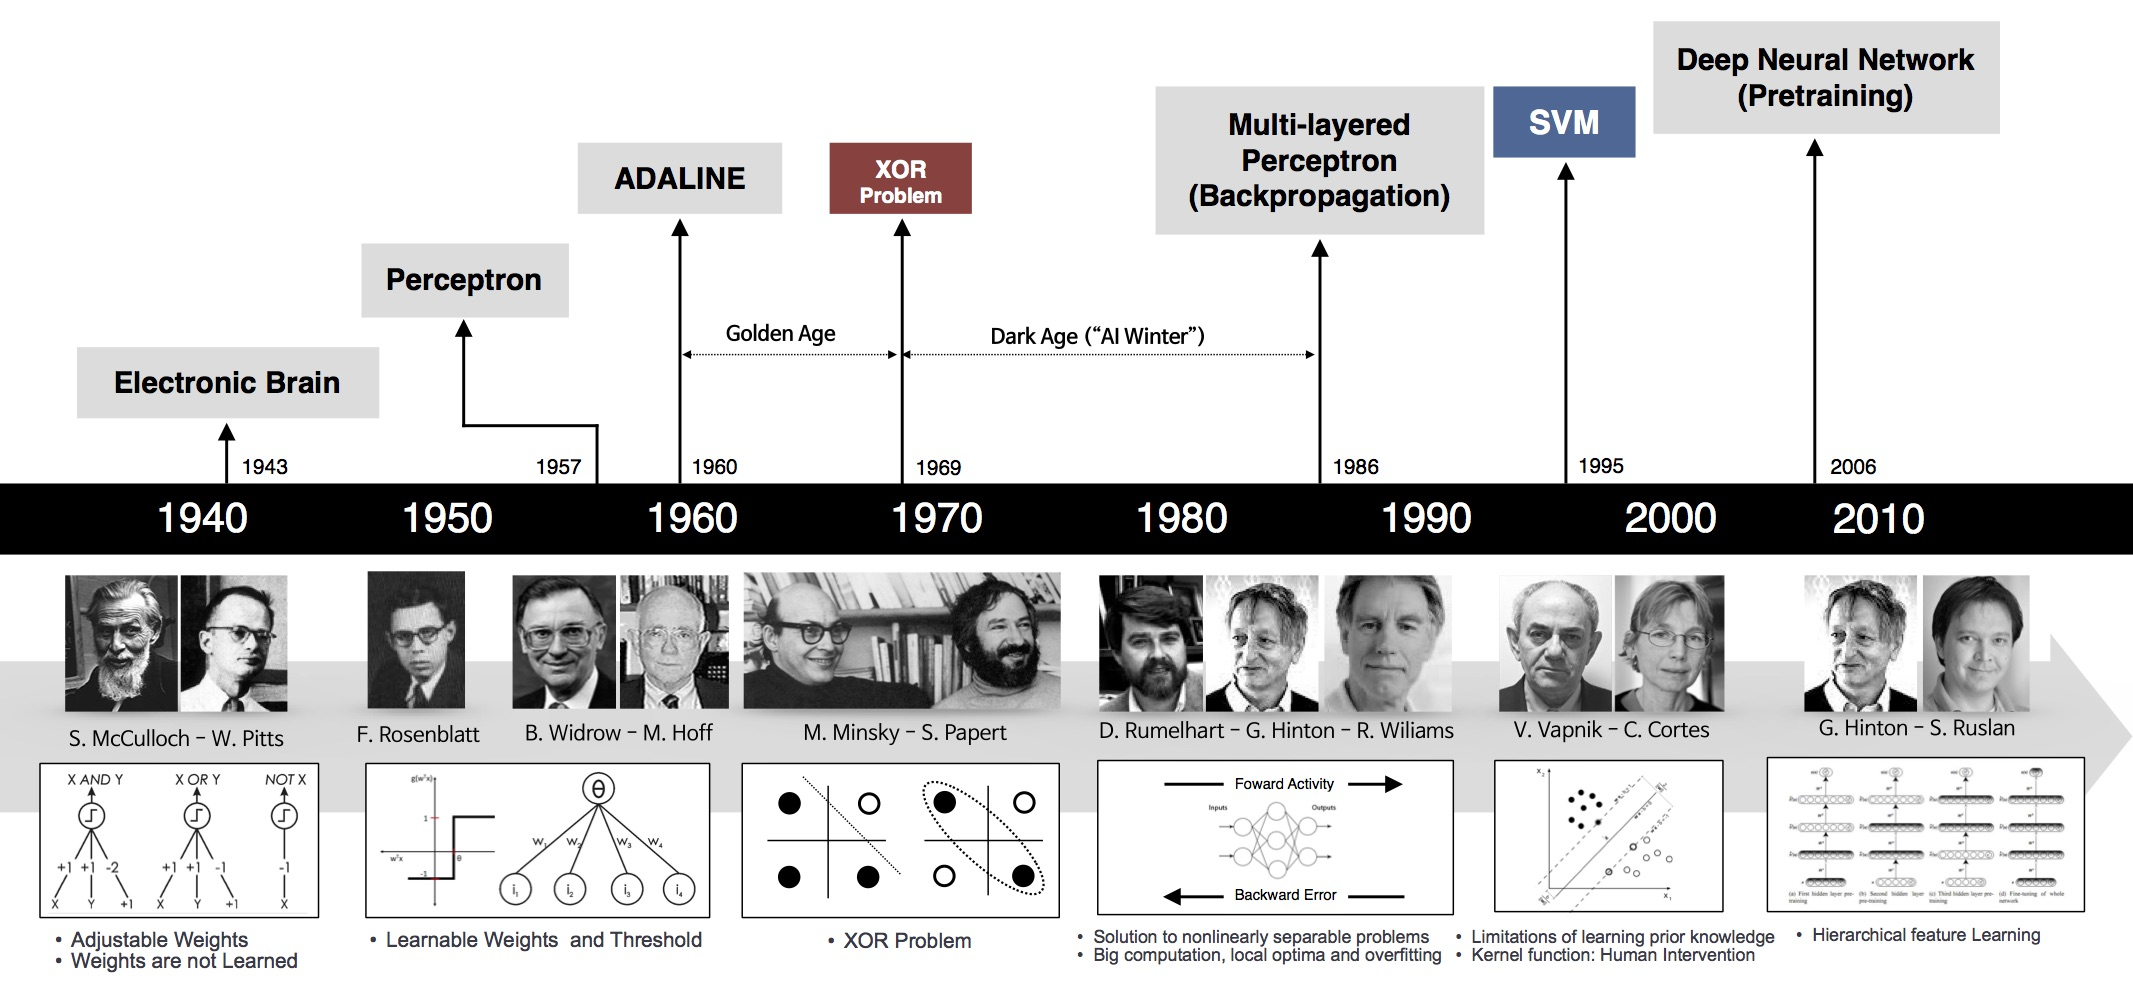
\includegraphics[width=1\linewidth]{imgs/nn_timeline}
\end{figure}
\end{frame}

% Neuron
\begin{frame}
  \vspace*{1cm}
  \textbf{Neuron:} The basic computational unit of the brain  \\
  \textbf{Walter Pitts and Warren McCulloch [1943]:}\\
  \textbf{Thresholded logic unit} (designed to mimic the way a neuron was thought to work) \\
  adjustable but \textit{not learned} weights \\
  \vspace*{-.5cm}
  \begin{eqnarray}
  \mbox{output} & = & \left\{ \begin{array}{ll}
  0 & \mbox{if } \sum_j w_j x_j \leq \mbox{ threshold} \\
  1 & \mbox{if } \sum_j w_j x_j > \mbox{ threshold}
  \end{array} \right.
  \nonumber
  \end{eqnarray}
  \hrulefill \\
  \begin{figure}[ht]
  	\centering
  	\subfloat[Biological Neuron]{%
  		\label{fig:first}%
  		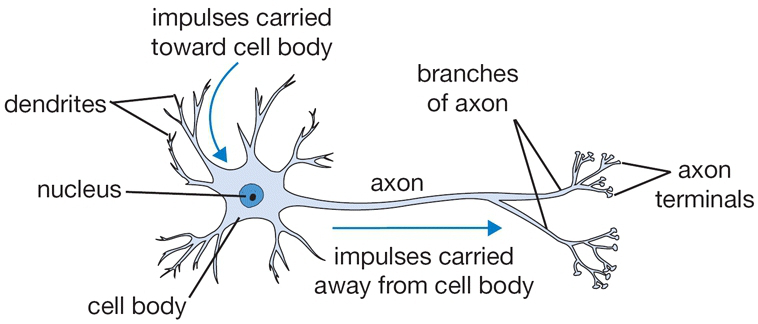
\includegraphics[width=0.5\linewidth]{imgs/neuron}}%
  	\qquad
  	\subfloat[Artificial Neuron]{%
  		\label{fig:second}%
  		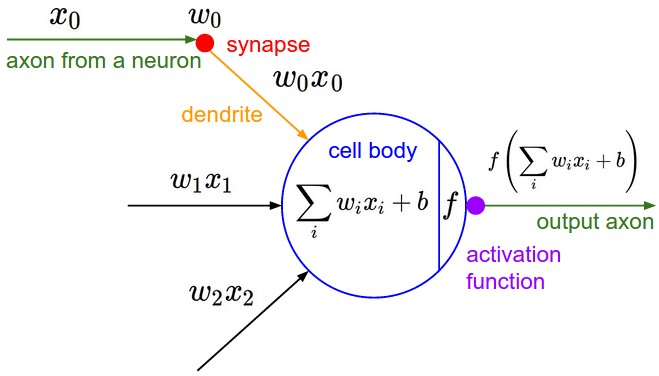
\includegraphics[width=0.4\linewidth]{imgs/artificial_neuron}}
  \end{figure}
\end{frame}

% Thresholded logic unit
\begin{frame}
  \vspace*{1cm}
  \textbf{Thresholded logic unit:} Maps inputs to 1 or 0 \\
  % \begin{multicols}{2}
    \begin{eqnarray}
    \mbox{output} & = & \left\{ \begin{array}{ll}
    0 & \mbox{if } \sum_j w_j x_j \leq \mbox{ threshold} \\
    1 & \mbox{if } \sum_j w_j x_j > \mbox{ threshold}
    \end{array} \right.
    \nonumber
    \end{eqnarray}

    % \columnbreak

    \begin{figure}
      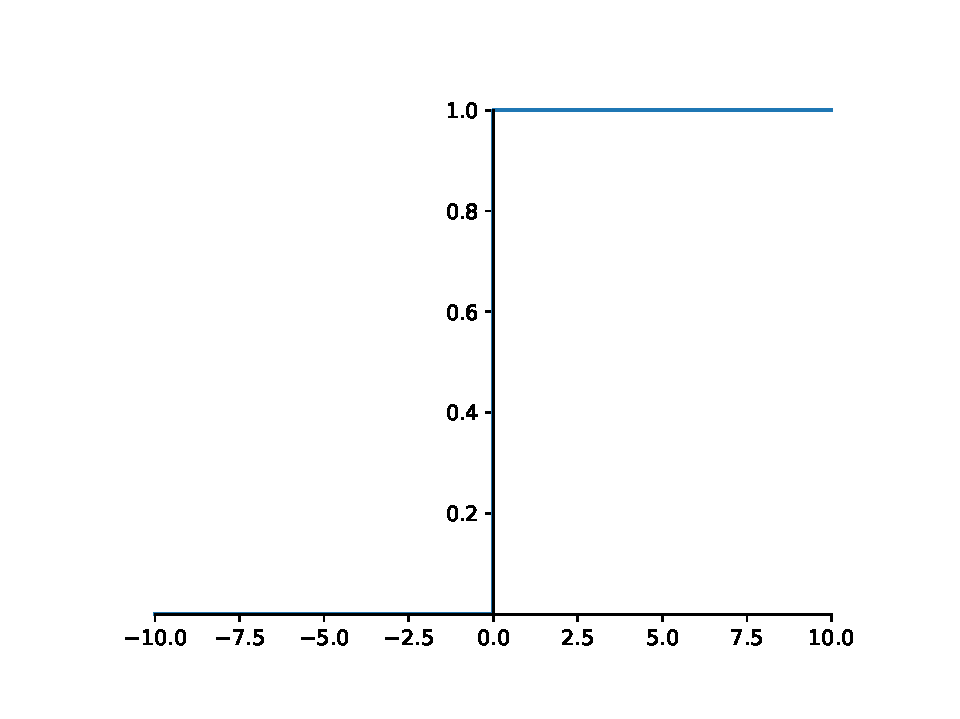
\includegraphics[width=.7\linewidth]{imgs/step.pdf}
    \end{figure}
  % \end{multicols}
\end{frame}

% Frank Rosenblatt’s “perceptron”
\begin{frame}
  \textbf{Frank Rosenblatt’s “perceptron” [1957]:} \\First real precursor to modern neural networks \\
  Developed \textbf{rule for learning weights}

  \vspace{-.5cm}
  \begin{figure}
    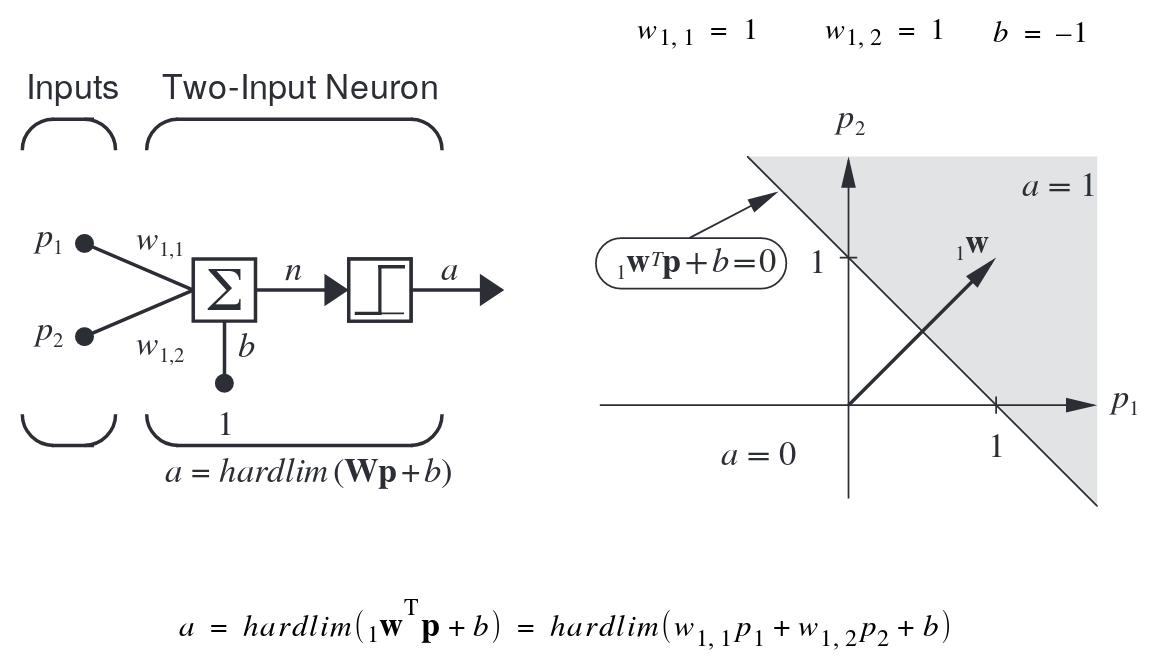
\includegraphics[width=.8\linewidth]{imgs/perceptron_1}
  \end{figure}
  \vspace{-.5cm}
  \textbf{Decision Boundary:} $w_{1,1}p_1 + w_{1,2}p_2 + b = 0$ \\
  \textbf{Linear equation:} $ax + by + c = 0$
\end{frame}

% Example - OR gate
\begin{frame}
  \vspace{1cm}
  \textbf{Supervised Learning} \\
  Network is provided with a set of examples of proper network behavior (inputs/targets)
  $$\{p_1, t_1\}, \{p_2, t_2\}, ..., \{p_Q, t_Q\}$$

  \textbf{Example - OR gate} \\ \hfill \break
  \vspace{-.6cm}
  \begin{figure}
    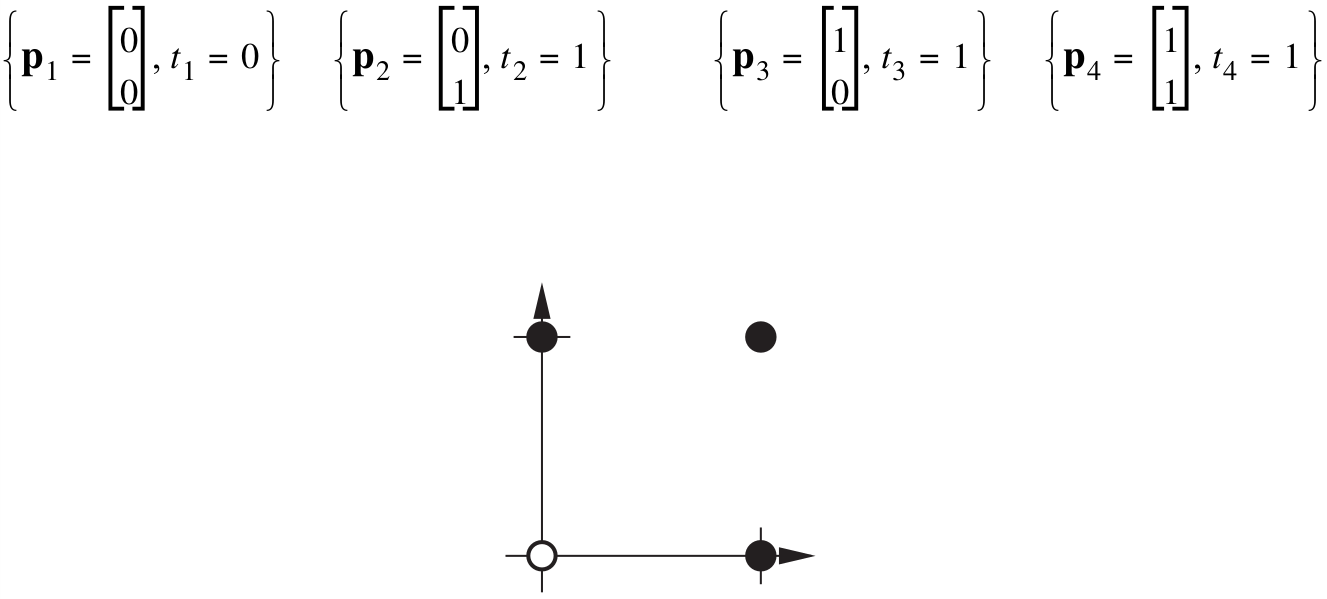
\includegraphics[width=.9\linewidth]{imgs/perceptron_or}
  \end{figure}
\end{frame}

% Example - OR gate
\begin{frame}
  \vspace{1cm}
  \textbf{Example - OR gate}
  \begin{figure}
    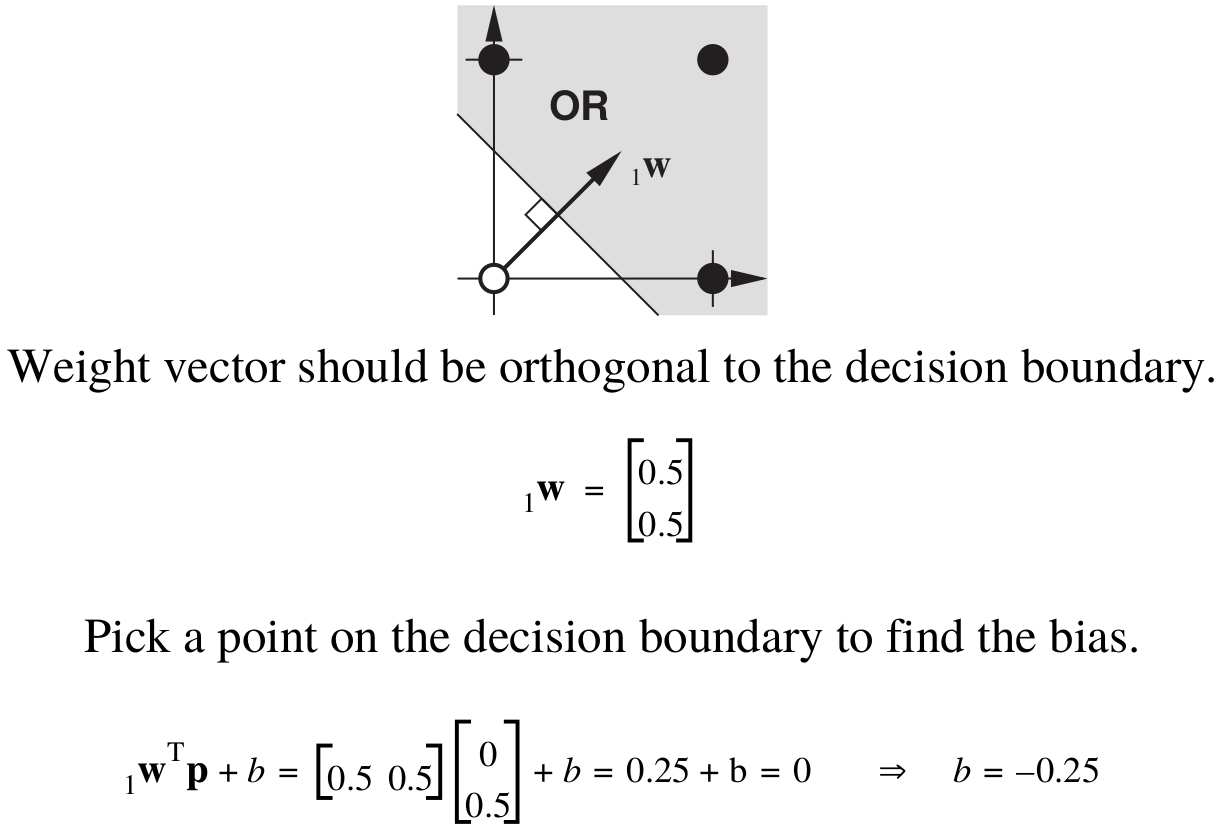
\includegraphics[width=.9\linewidth]{imgs/perceptron_or_2}
  \end{figure}
\end{frame}


\begin{frame}
  \vspace{1cm}
  \textbf{Learning Rule Test Problem}
  \begin{figure}
    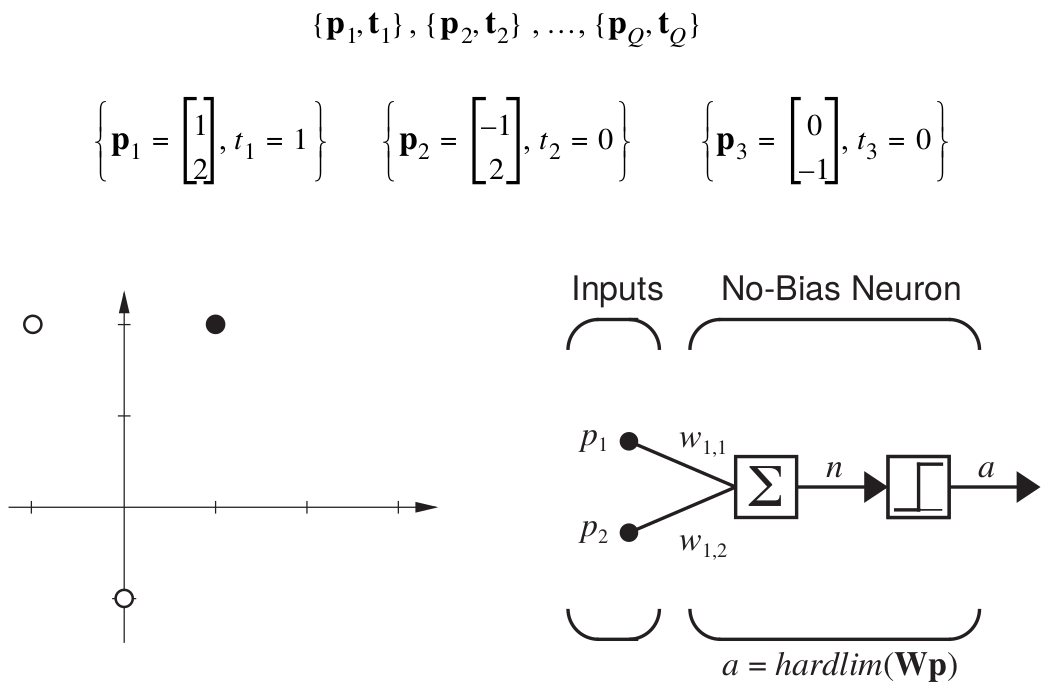
\includegraphics[width=.9\linewidth]{imgs/perceptron_ex_1}
  \end{figure}
\end{frame}

\begin{frame}
  \vspace{1cm}
  \textbf{Starting Point}
  \begin{figure}
    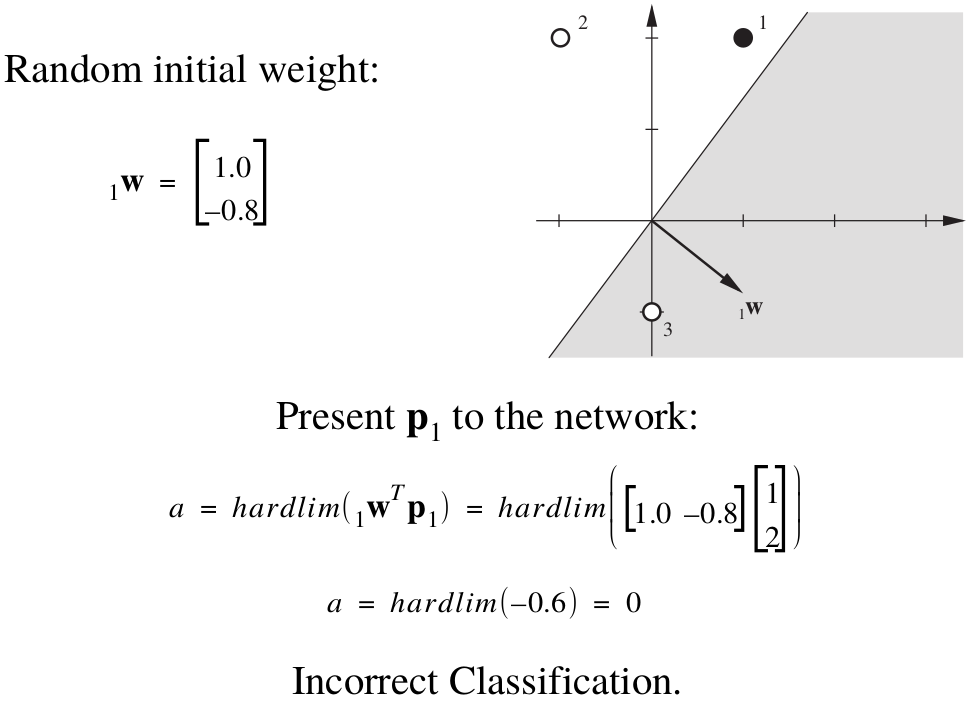
\includegraphics[width=.9\linewidth]{imgs/perceptron_ex_2}
  \end{figure}
\end{frame}

\begin{frame}
  \vspace{1cm}
  \textbf{Tentative Learning Rule}
  \begin{figure}
    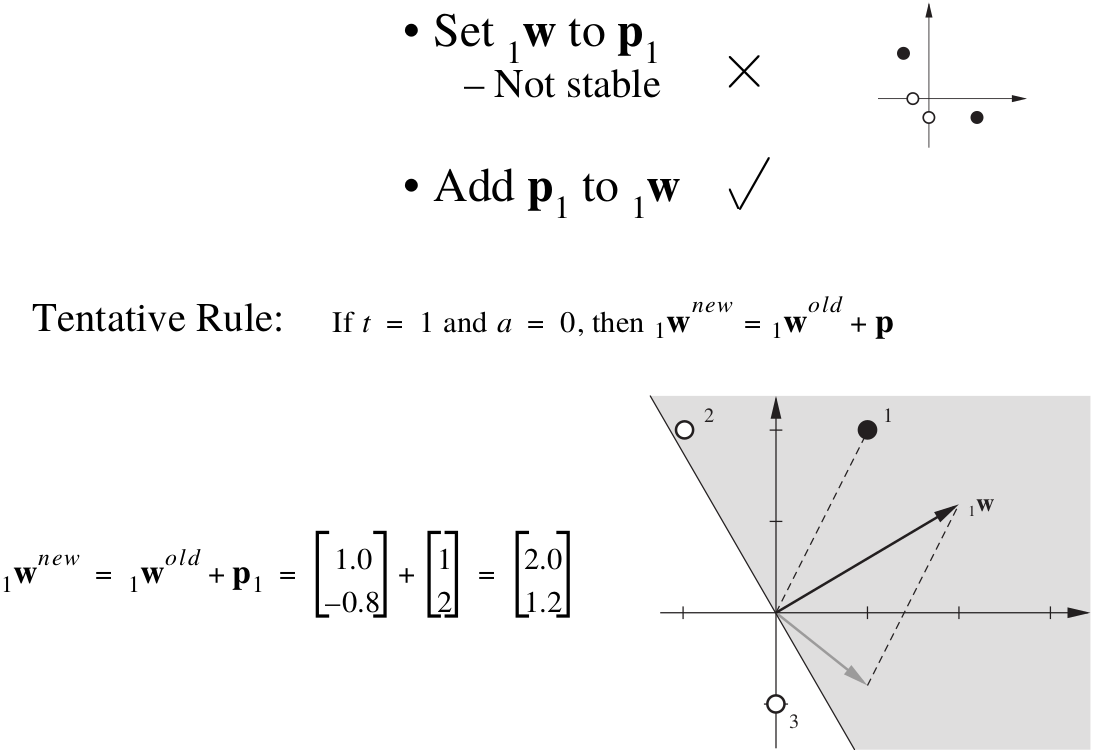
\includegraphics[width=.9\linewidth]{imgs/perceptron_ex_3}
  \end{figure}
\end{frame}

\begin{frame}
  \vspace{1cm}
  \textbf{Second Input Vector}
  \begin{figure}
    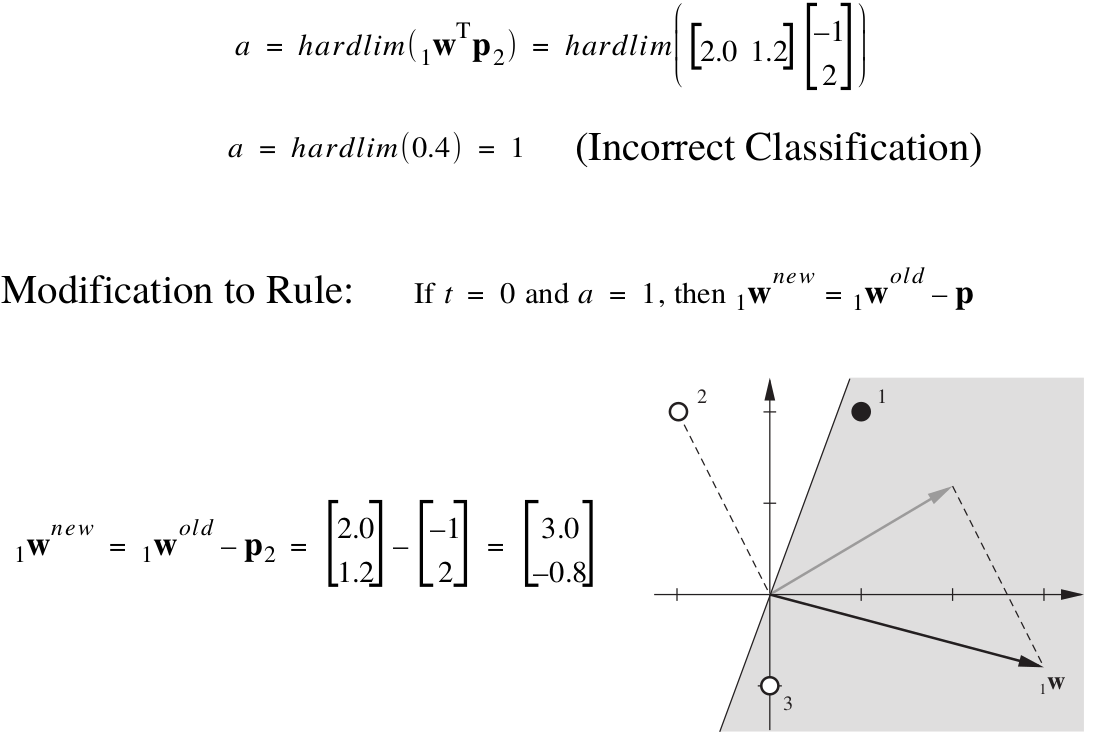
\includegraphics[width=.9\linewidth]{imgs/perceptron_ex_4}
  \end{figure}
\end{frame}

\begin{frame}
  \vspace{1cm}
  \textbf{Third Input Vector}
  \begin{figure}
    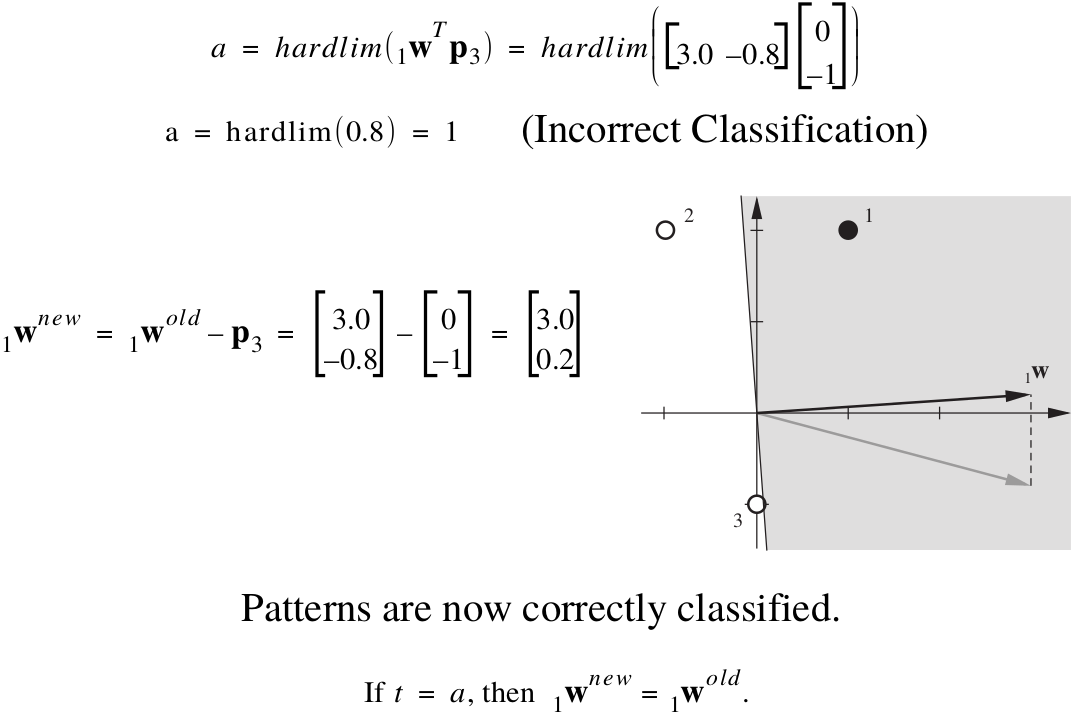
\includegraphics[width=.9\linewidth]{imgs/perceptron_ex_5}
  \end{figure}
\end{frame}

\begin{frame}
  \vspace{.5cm}
  \textbf{Unified Learning Rule}
  \begin{figure}
    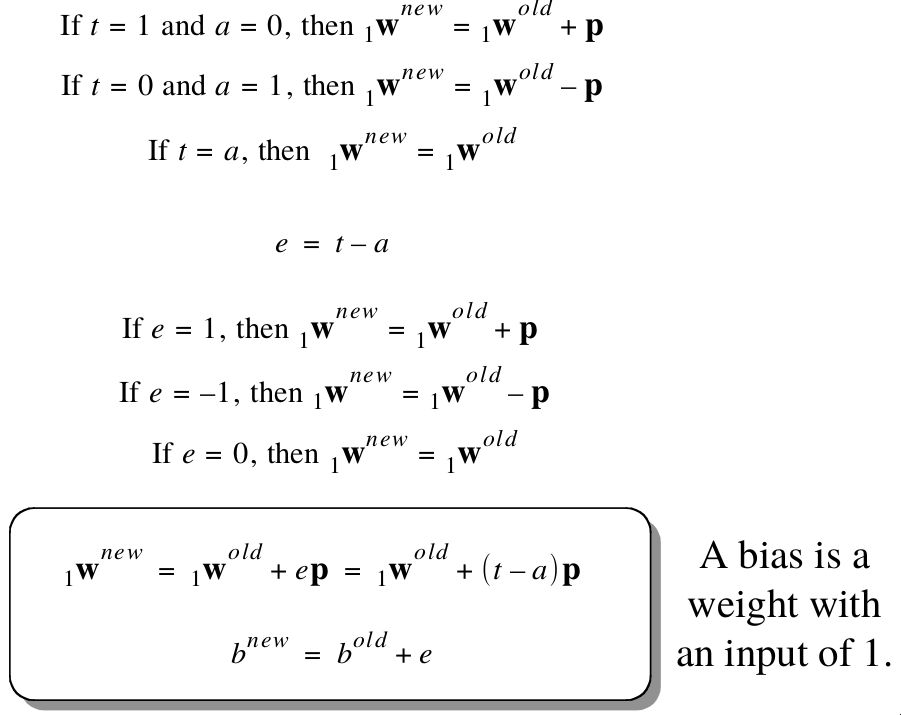
\includegraphics[width=.9\linewidth]{imgs/perceptron_ex_6}
  \end{figure}
\end{frame}

\begin{frame}
  \vspace{.5cm}
  \begin{figure}
    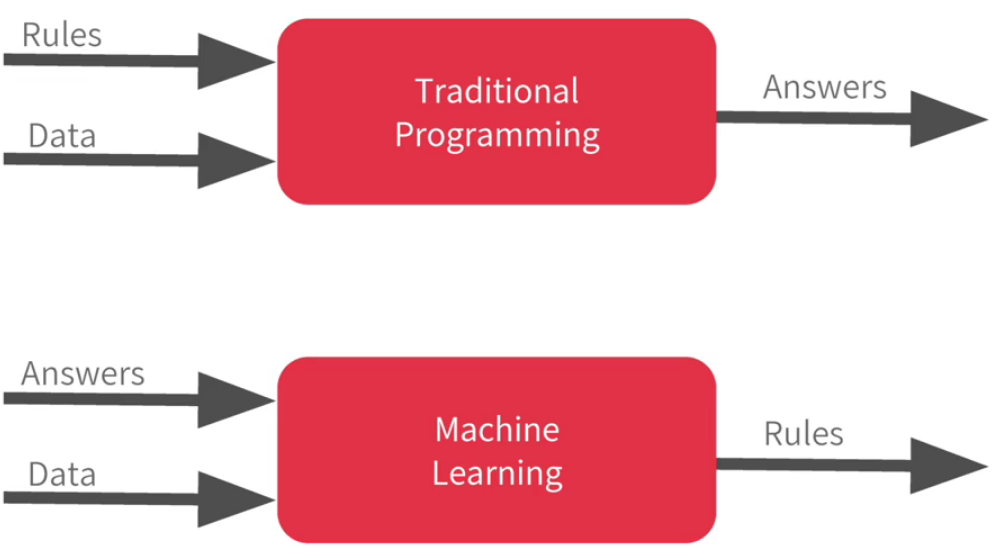
\includegraphics[width=.9\linewidth]{imgs/coursera_moroney/1}
  \end{figure}
\end{frame}


% \begin{frame}
% % $p_2 = -\frac{b}{w_{1,2}}$, if $p_1 = 0$ \qquad
% % $p_1 = -\frac{b}{w_{1,1}}$, if $p_2 = 0$
% \textbf{Perceptron's Learning Rule} \\ \hfill \break
% \centering
% If $t = 1$ and $\alpha = 0$, then $w^{new} = w^{old} + p$ \\
% If $t = 0$ and $\alpha = 1$, then $w^{new} = w^{old} - p$ \\
% If $t = \alpha$, then $w^{new} = w^{old}$ \\
%
% $$e = t - \alpha$$
% If $e = 1$, then $w^{new} = w^{old} + p$ \\
% If $e = -1$, then $w^{new} = w^{old} - p$ \\
% If $e = 0$, then $w^{new} = w^{old}$ \\ \hfill \break
%
% $w^{new} = w^{old} + ep = w^{old} + (t-\alpha)p$ \\
% $b^{new} = b^{old} + e$
%
% \end{frame}

\begin{frame}
  % \textbf{AND gate example} \\
  %
  % \[
  % p_1 =
  % \begin{bmatrix}
  %   0 \\
  %   0
  % \end{bmatrix}
  % , t_1 = 0
  % \quad
  % p2 =
  % \begin{bmatrix}
  %   0 \\
  %   1
  % \end{bmatrix}
  % , t_2 = 0 \quad
  % p_3 =
  % \begin{bmatrix}
  %   1 \\
  %   0
  % \end{bmatrix}
  % , t_3 = 0
  % \quad
  % p4 =
  % \begin{bmatrix}
  %   1 \\
  %   1
  % \end{bmatrix}
  % , t_4 = 1\]
  % \vspace{1cm}
  \textbf{Perceptron convergence theorem} \\ \hfill \break
  \textit{The perceptron learning rule will converge to a weight vector (not necessarily unique) that  gives  the  correct  response  for  all  training  patterns,  and it will do so in a finite number of steps.} \\ \hfill \break
  Rosenblatt was so confident that the perceptron would lead to true AI, that in 1959 he remarked: \\ \hfill \break
  \textit{[The perceptron is] the embryo of an electronic computer that [the Navy] expects will be able to walk, talk, see, write, reproduce itself and be conscious of its existence.}

\end{frame}


\begin{frame}

\vspace*{.5cm}
\textbf{Marvin Minsky and Seymor Papert - XOR problem [1969]} \\ \hfill \break
They showed that the perceptron was incapable of learning the simple exclusive-or (XOR) function. \\
They proved that it was theoretically impossible for it to learn such a function, no matter how long you let it train.\\

\textit{(this isn’t surprising to us, as the model implied by the perceptron is a linear one and the XOR function is nonlinear)} \\\hfill \break
At the time this was enough to kill all research on neural nets\\

% Along with the double-PhD wielding Seymor Papert, Minksy wrote a book entitled Perceptrons that effectively killed the perceptron, ending embryonic idea of a neural net. They showed that the perceptron was incapable of learning the simple exclusive-or (XOR) function. Worse, they proved that it was theoretically impossible for it to learn such a function, no matter how long you let it train. Now this isn’t surprising to us, as the model implied by the perceptron is a linear one and the XOR function is nonlinear, but at the time this was enough to kill all research on neural nets \\

\end{frame}

\begin{frame}
  \vspace{.5cm}
  \begin{figure}
    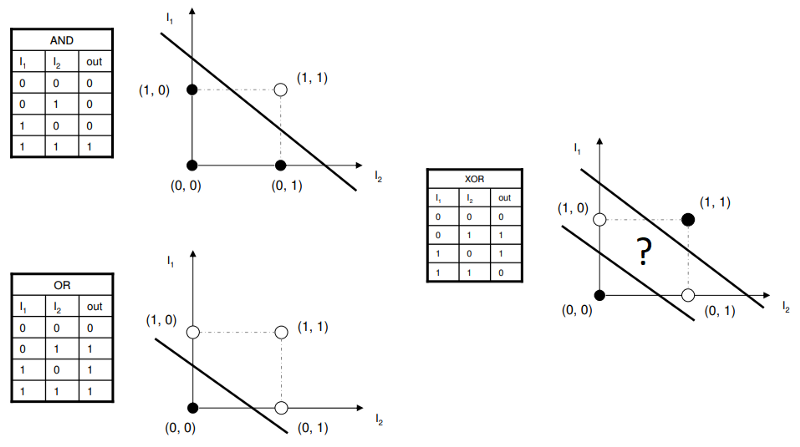
\includegraphics[width=1\linewidth]{imgs/xor_1}
  \end{figure}
\end{frame}

% AI Winter
\begin{frame}
  \vspace{.5cm}
  \begin{figure}
    
\includegraphics[width=.7\linewidth]{imgs/ai_winter}
  \end{figure}
\end{frame}

% XOR Solution???
\begin{frame}
  \vspace{.5cm}
  \centering
  \textbf{\Large{XOR Solution???}}
\end{frame}

% XOR Solution
\begin{frame}
  One single perceptron neuron: One decision boundary (hyperplane) \\
  Two perceptron neurons: Two decision boundaries \\
  \textbf{Multi Layer Perceptron (MLP)}

  \begin{multicols}{2}
    \begin{figure}
      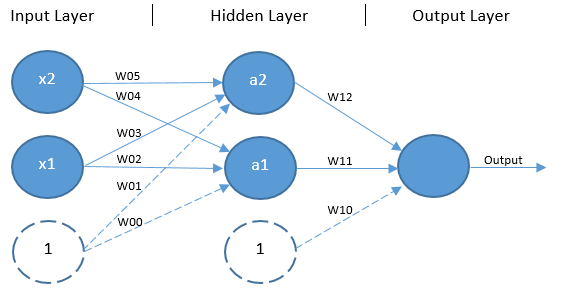
\includegraphics[width=1.2\linewidth]{imgs/mlp_1}
    \end{figure}

    \columnbreak

    \hfill \break
    \begin{figure}
      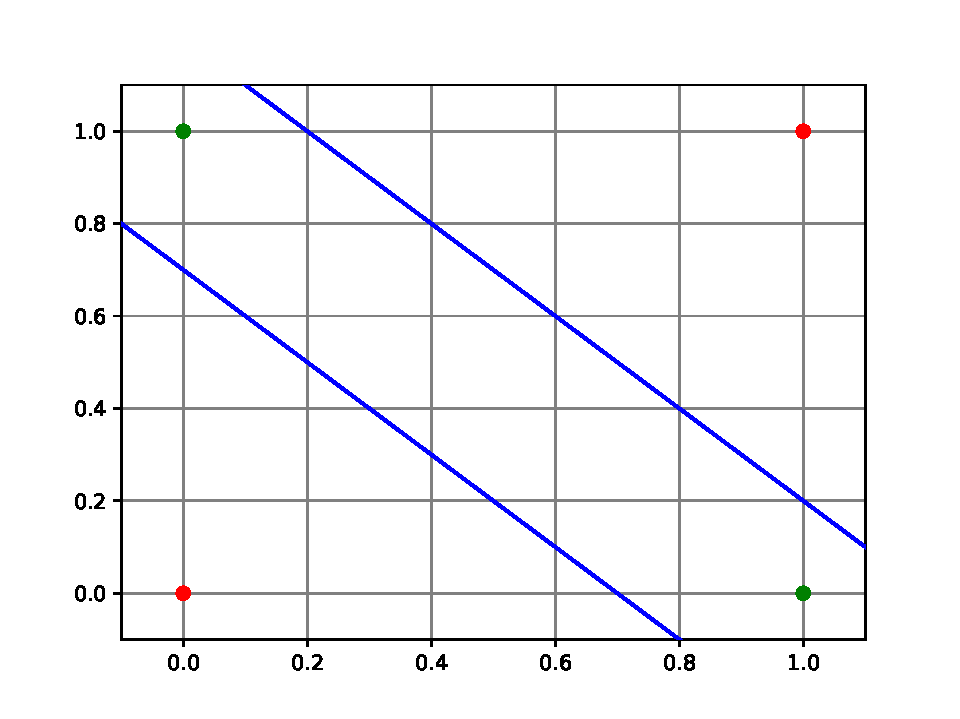
\includegraphics[width=.7\linewidth]{imgs/xor_sep-eps-converted-to.pdf}
    \end{figure}
  \end{multicols}
\end{frame}

% MLP - XOR as a logic gates
% \begin{frame}
%   \textbf{As a logic gates}
%
%   \begin{multicols}{2}
%     \begin{figure}
%       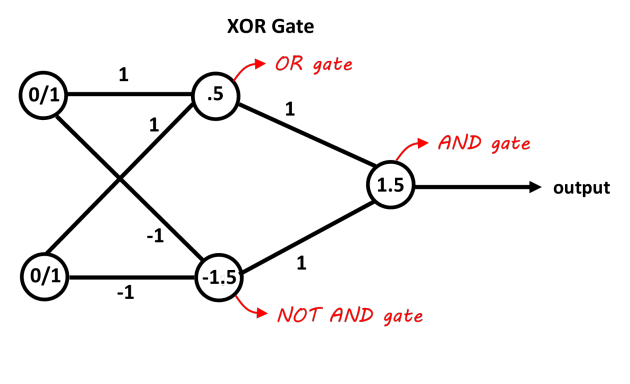
\includegraphics[width=1.2\linewidth]{imgs/mlp_2}
%     \end{figure}
%
%     \columnbreak
%
%     \hfill \break
%     \begin{figure}
%       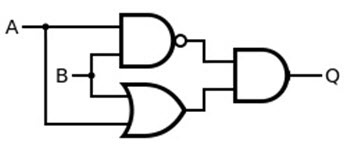
\includegraphics[width=.7\linewidth]{imgs/xor_nand_or}
%     \end{figure}
%   \end{multicols}
% \end{frame}

\begin{frame}
   A network of perceptrons can be used to simulate a circuit containing many NAND gates. And because NAND gates are universal for computation, it follows that perceptrons are also universal for computation. \\ \hfill \break
  \textit{In the mathematical theory of artificial neural networks, the universal approximation theorem states that a feed-forward network with a single hidden layer containing a finite number of neurons can approximate continuous functions on compact subsets of $R^n$, under mild assumptions on the activation function. The theorem thus states that simple neural networks can represent a wide variety of interesting functions when given appropriate parameters}
\end{frame}

\begin{frame}
  \vspace{.8cm}
  \textbf{The problem:} There was no equally powerfull rule (to the Perceptron's) for learning in networks with hidden units. \\
  \vspace{.5cm}

  \textbf{David. Rumelhard, Geoffrey. Hinton and Ronald. Williams - Learning Representations by back-propagating errors [1986]} \\
  (aka ``Backpropagation") \\

  \vspace{.5cm}
  \textbf{Perceptron's delta rule:} $\Delta_pw_{ji} = \eta (t_{pj} - o_{pj})i_{pi} = \eta \delta_{pj} i_{pi}$ \\ \hfill \break
  \textbf{How was this rule derived?} \\
  \textit{For linear units, this rule minimizes the squares of the differences between the actual and the desired output values summed over the output units and all pairs of input/output vectors.} $E = \sum E_p$
  $$ E_p = \frac{1}{2}\sum_j (t_{pj} - o_{pj})^2$$

\end{frame}

\begin{frame}
  \vspace{.5cm}
  \textbf{We have:} input and target data, network architecture \\
  \textbf{We want:} an algorithm which lets us find weights and biases so that the output from the network approximates y(x) (target $t$) for all training inputs x.  To quantify how well we're achieving this goal we define a cost function.

  $$ C(w, b) = \frac{1}{2n}\sum_x (t-\alpha)^2$$
  \textbf{$w$} the collection of all weights in the network, \textbf{$b$} all the biases, \textbf{$n$} the total number of training inputs, \textbf{$\alpha$} is the vector of outputs from the network when \textbf{$x$} is input, and the sum is over all training inputs, \textbf{$x$}.

  The output $\alpha$ depends on $x, w$ and $b$. \\
  We'll call $C$ the quadratic cost function (or mean squared error - MSE).

  $C(w,b)$ is non-negative. \\
  $C(w,b)$ becomes small i.e $C(w,b) \approx 0$ when $t \approx \alpha$.
\end{frame}

\begin{frame}

  $$ C(w, b) = \frac{1}{2n}\sum_x (t-\alpha)^2$$

  $ y = 2x + 4$ \\
  $x = [1, 2, 3, 4, 5, 6, 7, 8]$ \\
  $t = [6, 8, 10, 12, 14, 16, 18, 20]$ \\

  For $w = 3, b = 2$. \\
  $\alpha = [5, 8, 11, 14, 17, 20, 23, 26]$ \\ \hfill \break
  $C(w, b) = \frac{(6-5)^2 + (8-8)^2 + (10-11)^2 + ... + (20-26)^2}{16} = 5.75$ \\ \hfill \break

  The aim of our training algorithm will be to minimize the cost C(w,b) as a function of the weights and biases. In other words, we want to find a set of weights and biases which make the cost as small as possible. We'll do that using an algorithm known as \textbf{gradient descent}.
\end{frame}

\begin{frame}
   Minimize some function \\

   \begin{multicols}{2}
     The derivative of the function shows us the way the function changes. \\
     From Calculus is known that a function has a minimum (or maximum) value when its derivative at that point is zero.

     \begin{eqnarray}
     f\left(x + \epsilon\right) \approx f\left(x\right) + \epsilon f'\left(x\right)
     \nonumber
     \end{eqnarray}

     It is useful for minimizing the function because it tells us how to change $x$ in order to make a small improvement in $y$


     \columnbreak
     \begin{figure}
       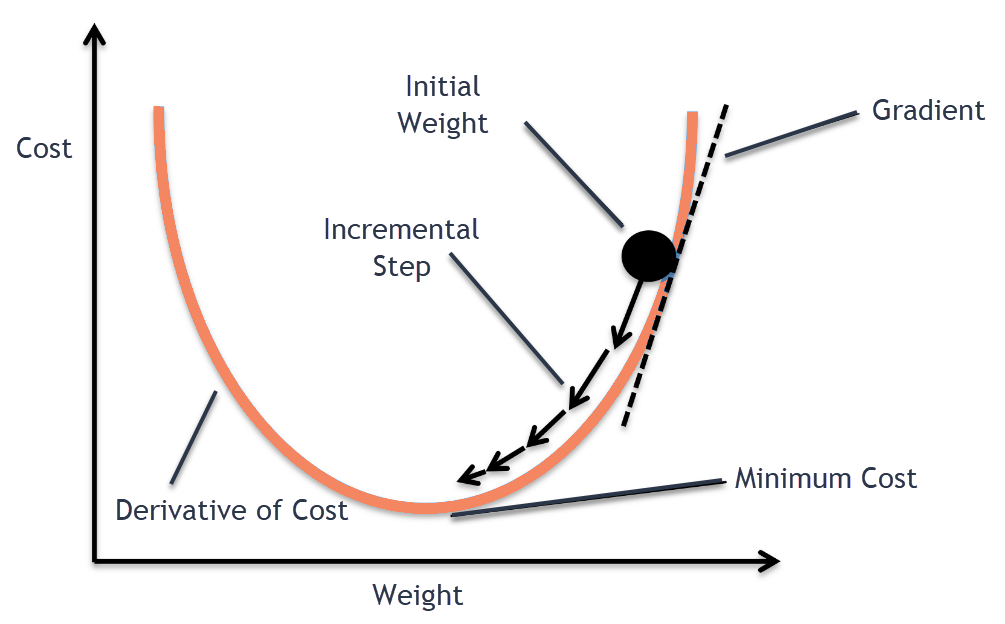
\includegraphics[width=1\linewidth]{imgs/gd_3}
     \end{figure}
  \end{multicols}
\end{frame}


\begin{frame}
  \begin{figure}
    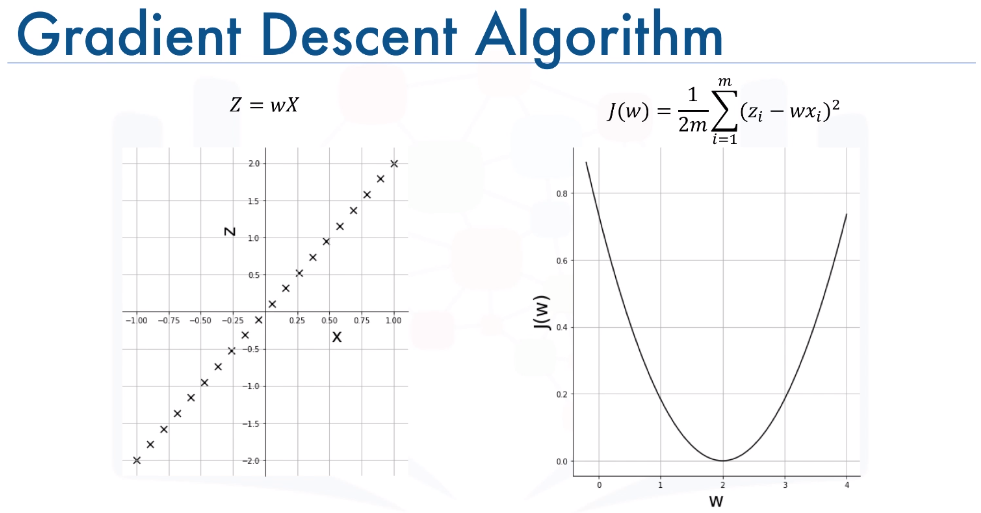
\includegraphics[width=1\linewidth]{imgs/edx_dl_keras/gd1}
  \end{figure}
\end{frame}

\begin{frame}
  \begin{figure}
    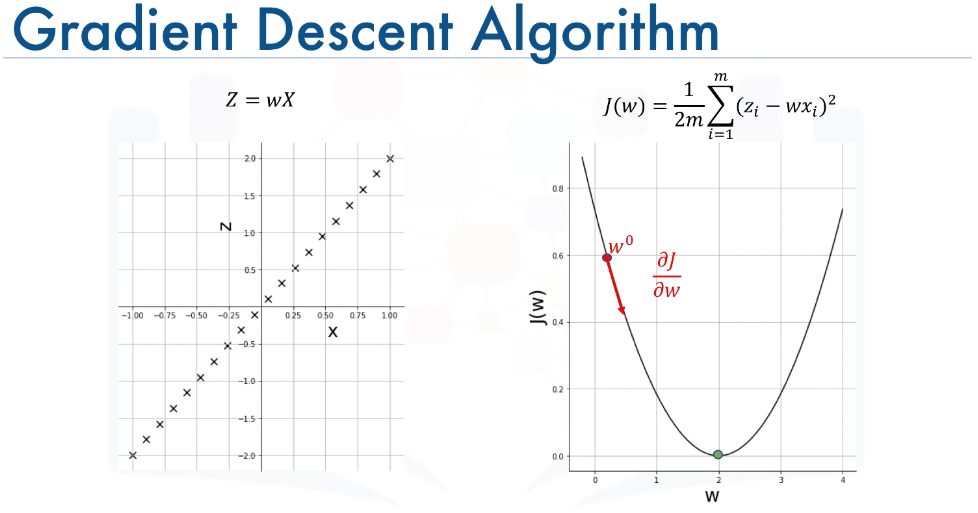
\includegraphics[width=1\linewidth]{imgs/edx_dl_keras/gd2}
  \end{figure}
\end{frame}

\begin{frame}
  \begin{figure}
    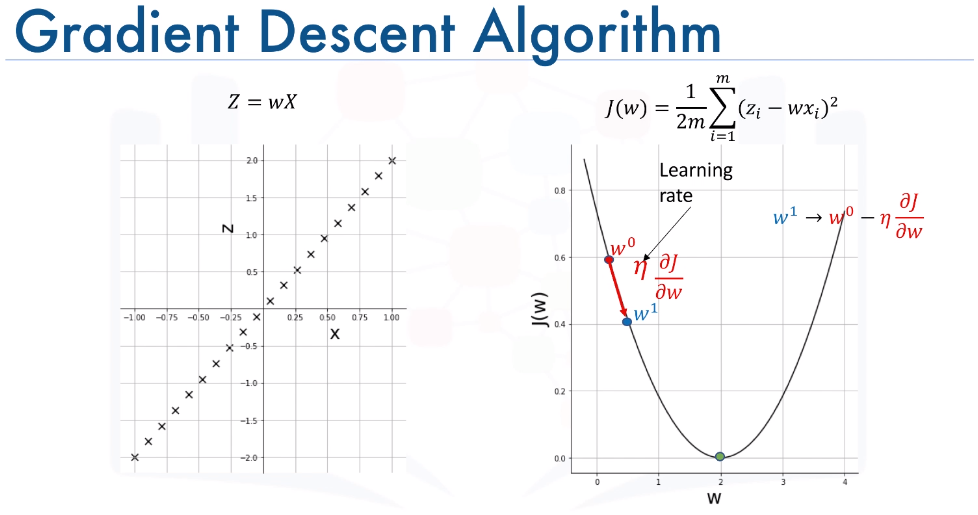
\includegraphics[width=1\linewidth]{imgs/edx_dl_keras/gd3}
  \end{figure}
\end{frame}

\begin{frame}
  \begin{figure}
    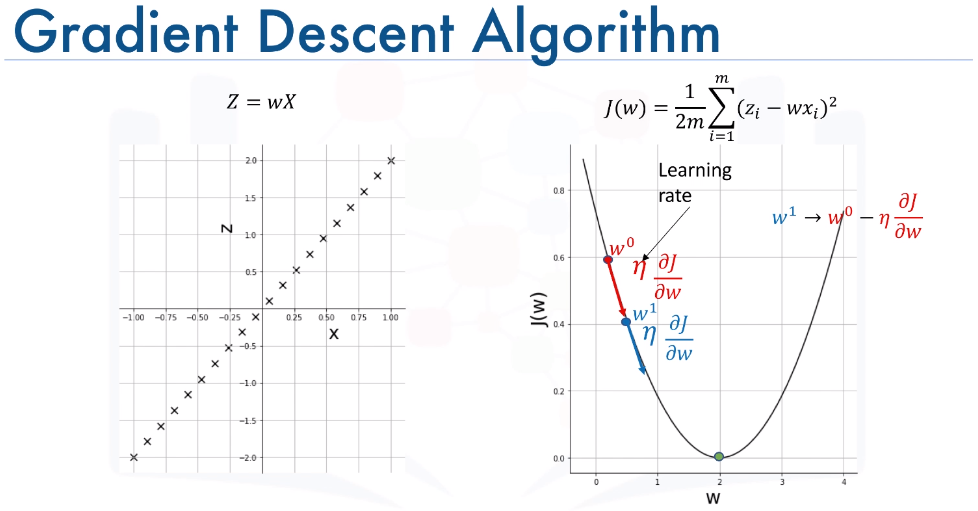
\includegraphics[width=1\linewidth]{imgs/edx_dl_keras/gd4}
  \end{figure}
\end{frame}

\begin{frame}
  \begin{figure}
    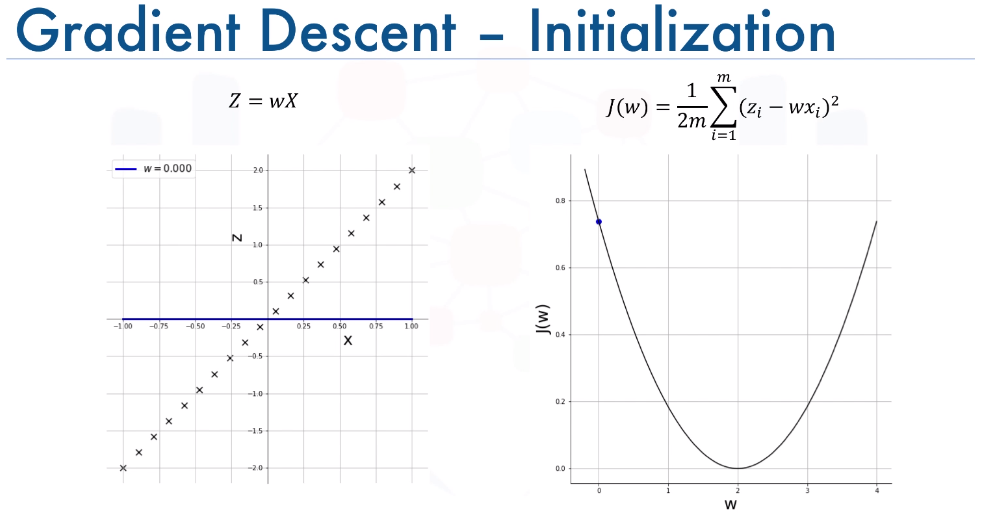
\includegraphics[width=1\linewidth]{imgs/edx_dl_keras/gd5}
  \end{figure}
\end{frame}

\begin{frame}
  \begin{figure}
    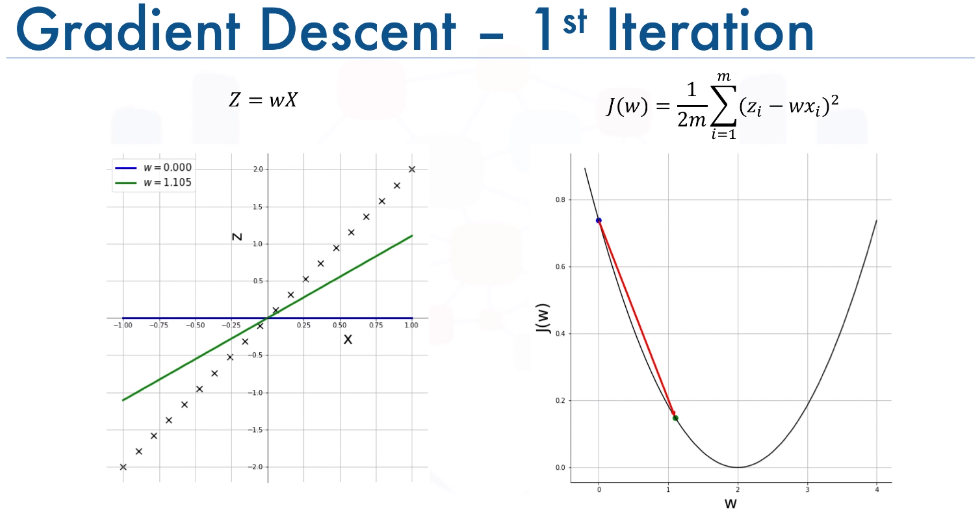
\includegraphics[width=1\linewidth]{imgs/edx_dl_keras/gd6}
  \end{figure}
\end{frame}

\begin{frame}
  \begin{figure}
    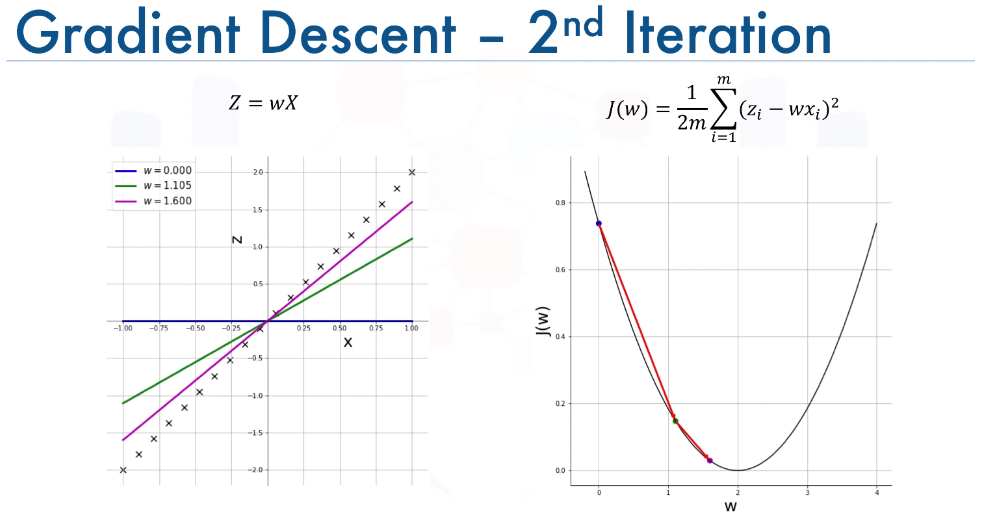
\includegraphics[width=1\linewidth]{imgs/edx_dl_keras/gd7}
  \end{figure}
\end{frame}

\begin{frame}
  \begin{figure}
    \includegraphics[width=1\linewidth]{imgs/edx_dl_keras/gd8}
  \end{figure}
\end{frame}

\begin{frame}
  \begin{figure}
    \includegraphics[width=1\linewidth]{imgs/edx_dl_keras/gd9}
  \end{figure}
\end{frame}

\begin{frame}
  \begin{figure}
    \includegraphics[width=1\linewidth]{imgs/edx_dl_keras/gd10}
  \end{figure}
\end{frame}

\begin{frame}
  \textbf{Critical points:}
  \begin{multicols}{2}
    The cost functions may have many local minima that are not optimal. \\
    This makes the optimization difficult, especially when the input is multidimensional.\\
    Usually we settle for finding a value of $f$ which is low, but not necessarily minimal.

  \columnbreak

    \begin{figure}
      \includegraphics[width=1\linewidth]{imgs/minima.pdf}
    \end{figure}
  \end{multicols}
\end{frame}

\begin{frame}
  \textbf{Multidimensional inputs:}
  \vspace{1cm}
  % \centering
  \begin{multicols}{2}
    \begin{figure}
      \includegraphics[width=1\linewidth]{imgs/gd_1}
    \end{figure}


    \columnbreak

  Usually we have multiple inputs and for that we use partial derivatives.\\
  There is a partial derivative for each input variable. \\
  The gradient of $f$ is the vector containing all the partial derivatives $\nabla_x f(x)$. Element $i$ of the gradient is the partial derivative of $f$ with respect to $x_i$. \\
  In multiple dimesions, critical points are these where every element of the gradient is equal to zero.
\end{multicols}
\end{frame}

\begin{frame}
  \textbf{Gradient descent:}\\
  To minimize $f$ we need to find the direction in which $f$ decreases the fastest.\\
  We can find the direction using the directional derivative. \\
  Moving in the direction of the negative gradient we can decrease $f$.
  This method is known as gradient descent.\\
  \begin{eqnarray}
    x' = x - \epsilon \nabla_xf(x)
    \nonumber
  \end{eqnarray}
  $\epsilon$ is the learning rate, a positive scalar determing the size of the step.\\
  There are many ways to set the value of this parameter\\


\end{frame}

\begin{frame}
  \vspace{.5cm}
  \textbf{Stochastic Gradient Descent:}\\
  Deep Learning needs large datasets which increase the computational cost of the gradient descent method.\\
  For the cost function:
  \begin{equation}
    J(\theta) = \frac{1}{m}\sum_{i=1}^{m} L(x^{(i)}, y^{(i)},\theta)
    \nonumber
  \end{equation}
  the gradient descent method needs to calculate the:
  \begin{equation}
    \nabla_\theta J(\theta) = \frac{1}{m}\sum_{i=1}^{m} \nabla_\theta L(x^{(i)}, y^{(i)},\theta)
    \nonumber
  \end{equation}
  which is $O(m)$
  However, the gradient is a prediction and because of that it can be an approximation using a small subset of the training dataset.\\
  This is the Stochastic Gradient Descent methods which is an extension of the gradient descent.
\end{frame}

\begin{frame}
  \textbf{So, how do we train a Multi Layer Perceptron?} \\
  \Large{$w_{1.1}^{new} = w_{1.1}^{old} - \eta \frac{\partial C}{\partial w_{1.1}}$}
  \begin{figure}
    \includegraphics[width=.8\linewidth]{imgs/mlp_backprop}
  \end{figure}
\end{frame}

\begin{frame}
  \vspace{1cm}
  \textbf{Back Propagation:} PROPAGATE the errors BACK to the input weights! \\
  \begin{figure}
    \includegraphics[width=.7\linewidth]{imgs/backprop_1}
  \end{figure}
  \textbf{Chain rule to the rescue!} \\
  $$\frac{\partial f}{\partial x} = \frac{\partial f}{\partial q} \frac{\partial q}{\partial x} =  \frac{\partial (q \cdot z)}{\partial q} \frac{\partial (x + y)}{\partial x} =
  z \cdot 1 = z = -4$$
  $$\frac{\partial f}{\partial z} = \frac{\partial (q \cdot z)}{\partial z} = q = 3$$
\end{frame}

\begin{frame}
  \vspace{0.6cm}
  \textbf{Sigmoid neurons - Sigmoid activation function} \\
  We want a small change in weight to cause only a small corresponding change in the output from the network. \\
  \textbf{Not possible with perceptrons!} - a small change in the weights or bias of any single perceptron in the network can sometimes cause the output of that perceptron to completely flip, say from 0 to 1
  \begin{figure}
    \includegraphics[width=.7\linewidth]{imgs/sigmoid_1}
  \end{figure}
\end{frame}

\begin{frame}
  \vspace{0.7cm}
  \begin{multicols}{2}
    The ouputs of the sigmoid neuron is NOT 0 or 1. \\
    $output = \sigma(w \cdot x + b)$, where $\sigma$ is the sigmoid function. \\
    $$\sigma(z) = \frac{1}{1 + e^{-z}} = \frac{1}{1 + exp(-\sum_j w_jx_j - b)}$$
    \columnbreak
    \begin{figure}
      \includegraphics[width=.7\linewidth]{imgs/sigmoid_2}
    \end{figure}
  \end{multicols}

  \begin{figure}[ht]
  	\centering
  	\subfloat{%

  		\includegraphics[width=0.45\linewidth]{imgs/ch-02-v4-06a}}%
  	\qquad
  	\subfloat{%
  		\includegraphics[width=0.45\linewidth]{imgs/ch-02-v4-06b}}%
  \end{figure}

\end{frame}

\begin{frame}
  \vspace{1cm}
  \begin{figure}
    \includegraphics[width=1\linewidth]{imgs/backprop_2}
  \end{figure}
  $q = w_0 \cdot x_0,$ \quad $p = w_1 \cdot x_1,$ \quad $s = q + p,$ \quad $t = w_2 + s,$ \quad $r = -t,$ \quad $u = e^r,$ \quad $v = u + 1$ and $z = \frac{1}{v}$ \\
  \Large{$\frac{\partial z}{\partial w_0} = \frac{\partial z}{\partial v}\frac{\partial v}{\partial u}\frac{\partial u}{\partial r}\frac{\partial r}{\partial t}\frac{\partial t}{\partial s}\frac{\partial s}{\partial q}\frac{\partial q}{\partial w_0} = $} \\
  \small{$-0.53 \cdot 1 \cdot 0.37 \cdot (-1) \cdot 1 \cdot 1 \cdot  x_0 = -0.1961 \approx -0.20$}
\end{frame}

\begin{frame}
  \vspace{1cm}
  \begin{figure}
    \includegraphics[width=1\linewidth]{imgs/backprop_3}
  \end{figure}
\end{frame}

\begin{frame}
  \vspace{0.6cm}

  \begin{figure}
    \includegraphics[width=.85\linewidth]{imgs/softmax_1}
  \end{figure}

  \begin{multicols}{2}
    \textbf{Softmax function} \\
  $$ \sigma (z)_i = \frac{e^{z_i}}{\sum_{j=1}^K e^{z_j}}$$
  \columnbreak
  \begin{figure}
    \includegraphics[width=.9\linewidth]{imgs/softmax_3}
  \end{figure}

  \end{multicols}
\end{frame}



\begin{frame}
  \vspace{.5cm}
  \begin{figure}
    \includegraphics[width=.8\linewidth]{imgs/softmax_2}
  \end{figure}

  \begin{multicols}{2}
    \begin{figure}
      \includegraphics[width=.9\linewidth]{imgs/categorical_1}
    \end{figure}
  \columnbreak
    \begin{figure}
      \includegraphics[width=.75\linewidth]{imgs/categorical_2}
    \end{figure}

  \end{multicols}

\end{frame}

\begin{frame}
  https://cs.stanford.edu/people/karpathy/convnetjs/demo/classify2d.html \\
\end{frame}

\begin{frame}
  \vspace{1cm}
  \textbf{Recap} \\
  \begin{itemize}
    \item[--] Neural Networks are made up of neurons that have learnable weights and biases.
    \item[--] Each neuron receives some inputs, performs a dot product and usually follows it with a non-linearity.
    \item[--] The whole network still expresses a single differentiable score function: from the raw input data on one end to class scores at the other - the network transforms the input through a series of hidden layers
    \item[--] Each hidden layer is made up of a set of neurons, where each neuron is fully connected to all neurons in the previous layer, and where neurons in a single layer function completely independently and do not share any connections.
    \item[--] The last fully-connected layer is called the “output layer” and in classification settings it represents the class scores.
    \item[--] And networks have a loss function on the last layer.
  \end{itemize}

\end{frame}

\begin{frame}
  Other activation functions \\
  tanh, relu, leaky relu
\end{frame}

\begin{frame}
  \textbf{Convolutional Neural Networks (CNNs} \\ \hfill \break
  \begin{itemize}
    \item[--] Convolutional Neural Networks are very similar to ordinary Neural Networks
    \item[--] BUT CNN architectures make the explicit assumption that the inputs are images
    \item[--] vastly reduce the amount of parameters in the network.
  \end{itemize}
\end{frame}

\begin{frame}
  \vspace{0.6cm}
  \begin{multicols}{2}
    Fully Connected neural nets can recognize images of handwritten digits.
    \columnbreak
    \begin{figure}
      \includegraphics[width=.65\linewidth]{imgs/digits}
    \end{figure}
  \end{multicols}
  \begin{figure}
    \includegraphics[width=.75\linewidth]{imgs/mlp_4}
  \end{figure}
  \textbf{Input:} 28 x 28 pixels = 784 neurons \\
  \textbf{Output:} 10 neurons (10 classes)
\end{frame}

\begin{frame}
  images aka 2D aka spatial structure \\
  BUT a FC model does not take into account this spatial structure of the images.

  Convolutional neural networks use three basic ideas:\\
  \begin{itemize}
    \item[--] local receptive fields
    \item[--] shared weights
    \item[--] pooling
  \end{itemize}
\end{frame}

\begin{frame}
  \vspace{0.6cm}
  \textbf{Local receptive fields} \\
  \begin{multicols}{2}
    Think of the input (image) as 28 x 28 square of neurons
    \columnbreak
    \begin{figure}
      \includegraphics[width=.6\linewidth]{imgs/cnn/cnn_1}
    \end{figure}
  \end{multicols}
  \begin{multicols}{2}
    We connect the inputs pixels to a layer of hidden neurons. \\
    Each neuron in the first hidden layer will be connected to a small region of the input neurons, e.g. a 5×5 region, corresponding to 25 input pixels.
    \columnbreak
    \begin{figure}
      \includegraphics[width=.8\linewidth]{imgs/cnn/cnn_2}
    \end{figure}
  \end{multicols}
\end{frame}

\begin{frame}
  \begin{itemize}
    \item[--] Each connection learns a weight.
    \item[--] The hidden neuron learns an overall bias.
    \item[--] We slide the local receptive field across the entire input image.
    \item[--] For each local receptive field, there is a different hidden neuron in the first hidden layer.
  \end{itemize}
   \textit{If we have a 28×28 input image, and 5×5 local receptive fields, then there will be 24×24 neurons in the hidden layer.}

  \begin{figure}
    \includegraphics[width=.6\linewidth]{imgs/cnn/cnn_3}
  \end{figure}
\end{frame}

\begin{frame}
  \vspace{0.6cm}
  \textbf{Shared weights and biases} \\ \hfill \break
  Each hidden neuron has a bias and 5 x 5 weights connected to its local receptive field. \\
  !!! Each of the 24 x 24 hidden neuron in the first hidden layer uses the smae weights and bias!
  \begin{eqnarray}
  \sigma\left(b + \sum_{l=0}^4 \sum_{m=0}^4  w_{l,m} a_{j+l, k+m} \right).
  \nonumber
  \end{eqnarray}
  where $\sigma$ is the activation function, $b$ is the shared bias, $w_{l,m}$ is the 5 x 5 array of shared weights and $a_{x,y}$ the input activation at position $x,y$. \\
  This 5 x 5 weight (+ bias) array is defines a \textbf{kernel} or \textbf{filter}.
\end{frame}

\begin{frame}
  \vspace{0.6cm}
  \textbf{What does this mean???} \\ \hfill \break
  All the neurons in the first hidden layer detect exactly the same \textbf{feature}. \\
  \textit{(think of the feature detected by a hidden neuron as the kind of input pattern that will cause the neuron to activate: it might be an edge in the image, for instance, or maybe some other type of shape.)}
  \begin{figure}
    \includegraphics[width=.6\linewidth]{imgs/cnn/example_filters}
  \end{figure}
  \small Example filters by Krizhevsky et al. Because these filters were learned using the first convolutional layer of the neural network, the represented features are simple, such as the edge orientation and frequency

\end{frame}

\begin{frame}
  \vspace{0.6cm}
  The filters extract features (e.g. edges). \\
  => \textbf{A filter is a feature detector!!!}

  For this reason, we sometimes call the map from the input layer to the hidden layer a \textbf{feature map}. \\

  To do image recognition we'll need more than one feature map. \\
  \begin{figure}
    \includegraphics[width=.6\linewidth]{imgs/cnn/cnn_4}
  \end{figure}

  3 feature maps means the network can detect 3 different kinds of features.
\end{frame}

\begin{frame}
  \vspace{0.6cm}
  The 20 images correspond to 20 different feature maps (or filters, or kernels).\\
  Each map is represented as a 5×5 block image, corresponding to the 5×5 weights in the local receptive field.\\
  Whiter blocks mean a smaller (typically, more negative) weight, so the feature map responds less to corresponding input pixels. \\
  Darker blocks mean a larger weight, so the feature map responds more to the corresponding input pixels.
  \begin{figure}
    \includegraphics[width=.6\linewidth]{imgs/cnn/kernels_1}
  \end{figure}
\end{frame}

\begin{frame}
  \vspace{0.6cm}
  \textbf{Sharing weights and biases greatly reduces the number of parameters involved!} \\ \hfill \break
  \textbf{CNN} \\
  5 x 5 (weights) + 1 (bias) = 26 parameters for each feature map. \\
  20 feature maps\\
  \textbf{Total:} 20 x 26=520 parameters defining the convolutional layer. \\ \hfill \break

  \textbf{FCN} \\
  28×28 = 784 input neurons \\
  30 hidden neurons \\
  \textbf{Total:} 784 x 30 (weights) + 30 (biases) = 23,550 parameters > 40 x 520!!!

\end{frame}

\begin{frame}
  \vspace{0.6cm}
  \textbf{Pooling} \\
  \begin{itemize}
    \item[--] Usually used immediately after convolutional layers.
    \item[--] Simplify the information in the output from the convolutional layer
  \end{itemize}
  \begin{figure}[ht]
  	\centering
  	\subfloat{%
  		\includegraphics[width=0.45\linewidth]{imgs/cnn/pool_1}}%
  	\qquad
  	\subfloat{%
  		\includegraphics[width=0.45\linewidth]{imgs/cnn/pool_2}}
  \end{figure}
  \textit{(Many pooling techniques: Max-Pooling, Avg-Pooling, L2-Pooling, etc.)}
\end{frame}

\begin{frame}
  \vspace{0.6cm}
  \textbf{We apply max-pooling to each feature map separately.} \\
  \begin{figure}
    \includegraphics[width=.7\linewidth]{imgs/cnn/pool_3}
  \end{figure}
  \textbf{Intuition:} Once a feature has been found, its exact location isn't as important as its rough location relative to other features. \\ \hfill \break
  This (among other things) makes CNNs invariant to image translation: move a picture of a cat a little ways, and it's still an image of a cat.
\end{frame}

\begin{frame}
  \vspace{0.6cm}
  \textbf{Putting it all together} \\
  28×28 input neurons (MNIST), followed by a convolutional layer using a 5×5 local receptive field and 3 feature maps. The result is a layer of 3×24×24 hidden feature neurons. \\
  Max-pooling layer, applied to 2×2 regions, across each of the 3 feature maps. \\
  The result is a layer of 3×12×12 hidden feature neurons. \\
  The final layer of connections in the network is a fully-connected layer - 10 output neurons.
  \begin{figure}
    \includegraphics[width=.7\linewidth]{imgs/cnn/cnn_5}
  \end{figure}
\end{frame}

\begin{frame}
  \begin{figure}
    \includegraphics[width=.7\linewidth]{imgs/cnn/vis_1}
  \end{figure}
  \begin{figure}
    \includegraphics[width=.7\linewidth]{imgs/cnn/vis_2}
  \end{figure}
\end{frame}

\begin{frame}
  Other loss functions \\
  binary cross entropy \\
  Categorical loss entropy \\
  Neirest Neighboor!!!
\end{frame}

% https://engmrk.com/lenet-5-a-classic-cnn-architecture/
\begin{frame}
  \vspace{0.6cm}
  \textbf{Le-Net 5 [1998]} \\
  Yann LeCun, Leon Bottou, Yosuha Bengio and Patrick Haffner proposed a neural network architecture for handwritten and machine-printed character recognition in 1990’s which they called LeNet-5.
  \begin{figure}
    \includegraphics[width=.9\linewidth]{imgs/cnn/lenet}
  \end{figure}
\end{frame}

\begin{frame}
  \vspace{0.6cm}
  \textbf{Le-Net 5 - First Layer} \\
  The input for LeNet-5 is a 32×32 grayscale image which passes through the first convolutional layer with 6 feature maps or filters having size 5×5 and a stride of one. The image dimensions changes from 32x32x1 to 28x28x6.
  \begin{figure}
    \includegraphics[width=.75\linewidth]{imgs/cnn/LeNet_Layer1}
  \end{figure}
\end{frame}

\begin{frame}
  \vspace{0.6cm}
  \textbf{Le-Net 5 - Second Layer} \\
  Then the LeNet-5 applies average pooling layer or sub-sampling layer with a filter size 2×2 and a stride of two. The resulting image dimensions will be reduced to 14x14x6.
  \begin{figure}
    \includegraphics[width=.75\linewidth]{imgs/cnn/LeNet_Layer2}
  \end{figure}
\end{frame}

\begin{frame}
  \vspace{0.6cm}
  \textbf{Le-Net 5 - Third Layer} \\
  Next, there is a second convolutional layer with 16 feature maps having size 5×5 and a stride of 1.
  \begin{figure}
    \includegraphics[width=.75\linewidth]{imgs/cnn/LeNet_Layer3}
  \end{figure}
\end{frame}

\begin{frame}
  \vspace{0.6cm}
  \textbf{Le-Net 5 - Fourth Layer} \\
  The fourth layer (S4) is again an average pooling layer with filter size 2×2 and a stride of 2. This layer is the same as the second layer (S2) except it has 16 feature maps so the output will be reduced to 5x5x16.
  \begin{figure}
    \includegraphics[width=.75\linewidth]{imgs/cnn/LeNet_Layer4}
  \end{figure}
\end{frame}

\begin{frame}
  \vspace{0.6cm}
  \textbf{Le-Net 5 - Fifth Layer} \\
  The fifth layer (C5) is a fully connected convolutional layer with 120 feature maps each of size 1×1. Each of the 120 units in C5 is connected to all the 400 nodes (5x5x16) in the fourth layer S4.
  \begin{figure}
    \includegraphics[width=.65\linewidth]{imgs/cnn/LeNet_Layer5}
  \end{figure}
\end{frame}

\begin{frame}
  \vspace{0.6cm}
  \textbf{Le-Net 5 - Sixth Layer} \\
  The sixth layer is a fully connected layer (F6) with 84 units.
  \begin{figure}
    \includegraphics[width=.75\linewidth]{imgs/cnn/LeNet_Layer6}
  \end{figure}
\end{frame}

\begin{frame}
  \vspace{0.6cm}
  \textbf{Le-Net 5 - Output Layer} \\
  Finally, there is a fully connected softmax output layer ŷ with 10 possible values corresponding to the digits from 0 to 9.
  \begin{figure}
    \includegraphics[width=.65\linewidth]{imgs/cnn/LeNet_Output_Layer}
  \end{figure}
\end{frame}

\begin{frame}
  \vspace{0.6cm}
  \textbf{Summary of LeNet-5 Architecture} \\
  \begin{figure}
    \includegraphics[width=.75\linewidth]{imgs/cnn/LeNEt_Summary_Table}
  \end{figure}
\end{frame}

\begin{frame}
  % https://www.learnopencv.com/understanding-alexnet/
  \vspace{0.6cm}
  \textbf{AlexNet} \\ \hfill \break
  In the year 2010 Deep Learning was... uncool... \\ \hfill \break
  That was the year ImageNet Large Scale Visual Recognition Challenge (ILSVRC) was launched. \\
  In 2012 Alex Krizhevsky, Ilya Sutskever, and Geoffrey E. Hinton published the paper ``ImageNet Classification with Deep Convolutional Neural Networks”. \\
  AlexNet was the winning entry in ILSVRC 2012.\\
  The paper used a CNN to get a Top-5 error rate (rate of not finding the true label of a given image among its top 5 predictions) of 15.3\%. The next best result trailed far behind (26.2\%).\\
  When the dust settled, Deep Learning was cool again.
\end{frame}

\begin{frame}
  \begin{figure}
    \includegraphics[width=.85\linewidth]{imgs/cnn/scholar_alexnet}
  \end{figure}
\end{frame}

\begin{frame}
  % https://www.youtube.com/watch?v=AgkfIQ4IGaM&list=PLqinEaadXCHZ7QT2KtEvibg_oHsHcx47H
  % https://www.youtube.com/watch?v=ghEmQSxT6tw
  t  \\
\end{frame}

\begin{frame}
  Autoencoders
\end{frame}

\begin{frame}
  U-Net
\end{frame}

\begin{frame}
\href{https://news.psu.edu/story/429727/2016/10/04/research/artificial-intelligence-could-help-farmers-diagnose-crop-diseases}{Artificial intelligence could help farmers diagnose crop diseases} \\
%
\href{https://www.youtube.com/watch?v=NlpS-DhayQA}{TensorFlow: an ML platform for solving impactful and challenging problems} \\

TensorFlow: an ML platform for solving impactful and challenging problems [\href{https://www.youtube.com/watch?v=NlpS-DhayQA}{link}] \\

Let there be Color! [\href{http://iizuka.cs.tsukuba.ac.jp/projects/colorization/extra.html}{link}] \\

Let there be Color! [\href{https://github.com/satoshiiizuka/siggraph2016_colorization}{github}]

refs \\
\href{https://www.sciencedaily.com/terms/artificial_intelligence.htm}{AI - Def.}
% https://engmrk.com/lenet-5-a-classic-cnn-architecture/
\end{frame}

\begin{frame}
  \vspace{1cm}
  ``AI talent is very scarse into this world" -Andrew Ng
  ethics and dangers in Deep Learning \\
  bias \\
  fake news \\
  deep fakes
\end{frame}

\end{document}
